\documentclass[twoside,a4paper,openright,12pt,tikz]{book}
\usepackage[T1]{fontenc}
\usepackage{amsfonts}
\usepackage{mathtools,amscd,amsthm}
\usepackage{tabularx}
\usepackage{amssymb,eucal,bezier,graphicx}
\usepackage{times}
\usepackage{subfig}
\usepackage[svgnames]{xcolor}
\usepackage{fancybox}
\usepackage{fancyhdr}
\usepackage{hyperref}
\usepackage{enumerate}
\usepackage{comment}
\usepackage[spanish]{babel}
\usepackage[utf8]{inputenc}
\usepackage{anysize}
\usepackage{listings}
\usepackage{etoolbox}
\usepackage{tikz}
\usepackage{float}

% Plantillas de código
\newcommand{\rstyle}{\lstset{ 
  language=R,                     % the language of the code
  basicstyle=\small\ttfamily, % the size of the fonts that are used for the code
  numbers=left,                   % where to put the line-numbers
  numberstyle=\tiny\color{Blue},  % the style that is used for the line-numbers
  stepnumber=1,                   % the step between two line-numbers. If it is 1, each line
                                  % will be numbered
  numbersep=5pt,                  % how far the line-numbers are from the code
  backgroundcolor=\color{white},  % choose the background color. You must add \usepackage{color}
  showspaces=false,               % show spaces adding particular underscores
  showstringspaces=false,         % underline spaces within strings
  showtabs=false,                 % show tabs within strings adding particular underscores
  frame=single,                   % adds a frame around the code
  rulecolor=\color{black},        % if not set, the frame-color may be changed on line-breaks within not-black text (e.g. commens (green here))
  tabsize=2,                      % sets default tabsize to 2 spaces
  captionpos=b,                   % sets the caption-position to bottom
  breaklines=true,                % sets automatic line breaking
  breakatwhitespace=false,        % sets if automatic breaks should only happen at whitespace
  keywordstyle=\color{RoyalBlue},      % keyword style
  commentstyle=\color{YellowGreen},   % comment style
  stringstyle=\color{ForestGreen},     % string literal style
     literate=%
         {á}{{\'a}}1
         {í}{{\'i}}1
         {é}{{\'e}}1
         {ý}{{\'y}}1
         {ú}{{\'u}}1
         {ó}{{\'o}}1
         {ñ}{{\~n}}1}}
         
\lstnewenvironment{erre}[1][]
{
\rstyle
\lstset{#1}
}
{}         

\definecolor{deepblue}{rgb}{0,0,0.5}
\definecolor{deepred}{rgb}{0.6,0,0}
\definecolor{deepgreen}{rgb}{0,0.5,0}

\newtoggle{InString}{}% Keep track of if we are within a string
\togglefalse{InString}% Assume not initally in string
\definecolor{majo}{HTML}{CD2626}
\newcommand*{\ColorIfNotInString}[1]{\iftoggle{InString}{#1}{\color{majo}#1}}%
\newcommand*{\ProcessQuote}[1]{#1\iftoggle{InString}{\global\togglefalse{InString}}{\global\toggletrue{InString}}}%


\DeclareFixedFont{\ttb}{T1}{txtt}{bx}{n}{12} % for bold
\DeclareFixedFont{\ttm}{T1}{txtt}{m}{n}{11}  % for normal

\newcommand{\pythonstyle}{\lstset{
  language=Python,                     % the language of the code
  basicstyle=\small\ttm, % the size of the fonts that are used for the code
  numbers=left,                   % where to put the line-numbers
  numberstyle=\tiny\color{DarkBlue},  % the style that is used for the line-numbers
  stepnumber=1,                   % the step between two line-numbers. If it is 1, each line
                                  % will be numbered
  numbersep=5pt,                  % how far the line-numbers are from the code
  backgroundcolor=\color{white},  % choose the background color. You must add \usepackage{color}
  showspaces=false,               % show spaces adding particular underscores
  showstringspaces=false,         % underline spaces within strings
  showtabs=false,                 % show tabs within strings adding particular underscores
  frame=single,                   % adds a frame around the code
  rulecolor=\color{black},        % if not set, the frame-color may be changed on line-breaks within not-black text (e.g. commens (green here))
  tabsize=2,                      % sets default tabsize to 2 spaces
  captionpos=b,                   % sets the caption-position to bottom
  breaklines=true,                % sets automatic line breaking
  breakatwhitespace=false,        % sets if automatic breaks should only happen at whitespace
  emph={range,len,print},          
  emphstyle=\ttb\color{deepred},
  keywordstyle=\color{RoyalBlue},      % keyword style
  commentstyle=\color{Grey},   % comment style
  stringstyle=\color{LimeGreen},     % string literal style
     literate=%
         {á}{{\'a}}1
         {í}{{\'i}}1
         {é}{{\'e}}1
         {ý}{{\'y}}1
         {ú}{{\'u}}1
         {ó}{{\'o}}1
         {ñ}{{\~n}}1
         {"}{{{\ProcessQuote{"}}}}1% Disable coloring within double q
         {'}{{{\ProcessQuote{'}}}}1% Disable coloring within single 
         {0}{{{\ColorIfNotInString{0}}}}1
    	 {1}{{{\ColorIfNotInString{1}}}}1
   	 	 {2}{{{\ColorIfNotInString{2}}}}1
   		 {3}{{{\ColorIfNotInString{3}}}}1
   		 {4}{{{\ColorIfNotInString{4}}}}1
   		 {5}{{{\ColorIfNotInString{5}}}}1
   		 {6}{{{\ColorIfNotInString{6}}}}1
   		 {7}{{{\ColorIfNotInString{7}}}}1
   		 {8}{{{\ColorIfNotInString{8}}}}1
   		 {9}{{{\ColorIfNotInString{9}}}}1
  }}
         
\lstnewenvironment{pythone}[1][]
{
\pythonstyle
\lstset{#1}
}
{}


\newcommand{\graphfromadj}[3][arc/.try]{
    \foreach [count=\r] \row in {#3}{
        \foreach [count=\c] \cell in \row{
            \ifnum\cell=1%
                \draw[arc/.try=\cell, #1] (#2\r) edge (#2\c);
            \fi
        }
    }
}

\newcommand{\weigthgraphfromadj}[3][draw,->]{
    \foreach [count=\r] \row in {#3}{
        \foreach [count=\c] \cell in \row{
            \if0\cell%
            \else
                \draw[arc/.try=\cell, #1] (#2\r) edge node[arc label/.try=\cell]{\cell} (#2\c);
            \fi
        }
    }
}


\marginsize{3.25cm}{3.25cm}{3cm}{3cm}

\newtheorem{defi}{Definici\'on}[section]
\newtheorem{ej}{Ejemplo}[section]
\newtheorem{ejs}{Ejemplos}[section]
\newtheorem{prop}{Proposici\'on}[section]
\newtheorem{nota}{Nota}[section]
\newtheorem{notac}{Notación}[section]
\newtheorem{rem}{Observaci\'on}[section]
\newtheorem{thm}{Teorema}[section]
\newtheorem{cor}{Corolario}[section]
\newtheorem{lem}{Lema}[section]
\newtheorem*{dem}{Demostración}

\providecommand{\abs}[1]{\left|{#1}\right|}
\providecommand{\conv}[1]{\overset{#1}{\longrightarrow}}
\providecommand{\convcs}{\xrightarrow{CS}}
\providecommand{\conve}{\xrightarrow{e}}
\providecommand{\func}[2]{\colon{#1}\longrightarrow{#2}}
\newcommand{\efe}{\hat{f}}
\newcommand{\R}{\mathbb{R}}
\newcommand{\D}{\mathbb{D}}
\newcommand{\Z}{\mathbb{Z}}
\newcommand{\N}{\mathbb{N}}
\newcommand{\E}{\mathbb{E}}
\newcommand{\fn}{\hat{f}_{0N}}
\newcommand{\X}{\overline{X}}
\newcommand{\dis}{\displaystyle}
\providecommand{\norm}[1]{\left\lVert#1\right\rVert}
\providecommand{\posi}[1]{\left[#1\right]^+}

% IRENITA--------------------------------
\renewcommand{\headrulewidth}{0.4pt} 
\fancyhead[RO,LE]{\thepage} 
\fancyhead[LO]{\nouppercase{\leftmark}}
\fancyhead[RE]{\nouppercase{\rightmark}}
\fancyfoot{}
\newcommand{\va}{\hat{\vartheta}_N}
\pagestyle{fancy}
% --------------------------------------

\setcounter{secnumdepth}{3}
\setcounter{tocdepth}{3}


\begin{document}
% ---------------------PORTADA
\begin{titlepage}

\vspace*{1in}
\begin{center}
\vspace*{-1in}
\begin{figure}[htb]
\begin{center}
\begin{large}
TRABAJO FIN DE MÁSTER\\
\end{large}
\rule{80mm}{0.1mm}\\
\vspace*{0.1in}
\end{center}
\end{figure}
\begin{large}
\end{large}

\vspace*{0.2in}
\begin{Large}
{\huge \bfseries El problema paramétrico del emparejamiento en grafos y
problema de emparejamiento con dos objetivos}\\[2cm]
\end{Large}

\begin{center} \Large
\emph{Presentado por:}\\
\textsc{ \bf{Rafael González López}}
\end{center}

\vspace*{0.2in}
\begin{center} \large
\emph{Supervisado por:} \\
\textsc{Dr.~Justo Puerto Albondoz}\\
\end{center}
\vspace*{0.2in}

\centering
\includegraphics[width =7cm]{logo}



\begin{large}
\centering
FACULTAD DE MATEMÁTICAS \\
\end{large} 

\begin{large}
Departamento de Estadística e Investigación Operativa\\
\end{large}


\begin{large}
\centering
Sevilla, Junio 2019\\
 \end{large}
\end{center}


\end{titlepage}

\newpage
\thispagestyle{empty}
%------------------------------------------------------------------------

\tableofcontents
\newpage
\thispagestyle{empty}

\chapter*{Abstract}
\addcontentsline{toc}{chapter}{Abstract}
The minimum (maximum) matching problem is a fundamental problem in combinatorial optimization. The special structure of matching found by Edmonds allows to use different approximations. The idea of this work is to present a general insight of the matching problem, different sorts of algorithms for solving its original and the bi-objective formulations and a computational approach. 

In section 1 we describe the problem, its applications and the Grötschel-Holland algorithm (for solving using linear programming). In section 2 we introduce the theoretical background necessary for understanding the SAP algorithm and the sensitive analysis. In section 3 we implement some methods in Python 3.7 with Gurobi to study their computational properties and sensitive analysis.
\newpage
\thispagestyle{empty}

\chapter*{Introducci\'on}\label{cap.introduccion}
\addcontentsline{toc}{chapter}{Introducción}
El problema del emparejamiento es uno de las cuestiones clásicas de la Programación Matemática. En este trabajo desarrollamos un extenso análisis sobre el trasfondo teórico de ciertos métodos para resolverlo, tanto en su formulación original, como en la formulación biobjetivo.

Tras una presentación inicial del problema, presentamos una primera aproximación a la resolución del problema mediante la Programación Lineal conocida como el algoritmo de Grötschel-Holland. Seguidamente, veremos numerosas aplicaciones que motivan el interés del problema.

En el segundo capítulo nos centramos en los conceptos y la estructura intrínseca del problema del emparejamiento, la cuál nos permite finalmente detallar el algoritmo del SAP. Además, presentamos el método de reoptimización propuesto por Derigs para este algoritmo.

Finalmente, dedicamos un epígrafe a realizar un análisis computacional. Implementamos en Python 3.7 distintos métodos de resolución del problema del emparejamiento con el fin de reportar una comparativa entre ellos. Finalmente, llevamos a cabo un análisis de sensibilidad del problema original y la versión biobjetivo.
\newpage
\thispagestyle{empty}
\chapter{El problema del emparejamiento}
El problema del emparejamiento es uno de los problemas clásicos de la optimización combinatoria. Representa uno de los momentos célebres en la historia de la optimización por ser el primer problema de Programación Entera, descontando aquellos que se resuelven usando la relajación lineal, en ser resuelto en tiempo polinomial. El caso bipartito puede verse como un problema de asginación y fue resuelto en tiempo polinómico por Harowld W. Kuhn con su famoso algoritmo húngaro en 1955 \cite{kuhn}, predecesor de los algoritmos dual-primal. Sin embargo, hubo que esperar hasta 1961 para que Jack Edmonds descubriera la solución del caso general. En su trabajo original (publicado en 1965 \cite{edmond}) no solamente caracterizó linealmente el poliedro del matching -abriendo el camino para métodos basados en el simplex- sino que utilizando estructura especial del problema construyó un algoritmo iterativo denominado \textit{algoritmo de blossom} que resuelve el problema polinomialmente.

\section{El problema del $b$-emparejamiento}
Dado que nuestro objetivo es el estudio paramétrico del problema del emparejamiento y la versión multiobjetivo del mismo, comenzamos este trabajo exponiendo en qué consiste el problema del ejemparejamiento o problema del \textit{matching}. Para ello, comenzamos definiendo algunos conceptos básicos en el marco de la teoría de grafos.
\begin{defi}
Sea $G=(V,E)$ un grafo y sea $S \subset V$, definimos $\delta(S)$ como el conjunto de aristas con un único extremo en $S$. En el caso de un conjunto unitario $\{i\}$, denotamos $\delta(i):=\delta(\{i\})$. Usualmente se denomina \textbf{grado del vértice $i$} al cardinal de $\delta(i)$. Definimos además $\gamma(S)$ como el conjunto de aristas que tienen ambos extremos en $S$.
\end{defi}

En adelante consideramos siempre $G=(V,E)$ un grafo no dirigido. El problema del \textit{matching} consiste en encontrar un subconjunto $M\subset E$ con la propiedad de que en el subgrafo inducido $G(M)=(V,M)$ ningún vértice tenga grado mayor que $1$, es decir, que ninguna arista tenga vértices en común con otra. Naturalmente, este problema es fácilmente generalizable al problema del $b$-emparejamiento o $b$-\textit{matching}, en el cual cada vértice $v$ debe tener un grado no mayor que $b_v$, donde $b_v$ es un entero positivo. El problema original pasaría a ser el caso particular en el que $b_v = 1$ $\forall v \in V$.

\begin{defi}
Sea $G=(V,E)$ un grafo y sea $M\subset E$ un $b$-emparejamiento. Diremos que $M$ es un \textbf{emparejamiento perfecto} si $|\delta(v)|=b_v$ $\forall v \in V$, es decir, si las restricciones se verifican con igualdad.
\end{defi}
Para cada $(u,v)\in E$ podemos considerar el peso o coste $c_{uv}$ asociado. Dependiendo del contexto en el que estemos trabajando estos pesos pueden ser números reales, reales positivos, enteros no negativos, etc. En este trabajo consideraremos que los costes son reales no negativos. Dado un conjunto de aristas $E'\subset E$, tiene sentido considerar
$$
c(E')=\sum_{(u,v)\in E'} c_{uv}
$$
El problema del $b$-emparejamiento de coste máximo o \textit{weighted $b$-matching problem} consiste en encontrar el $b$-emparejamiento que maximiza la función $c(\cdot)$. Si nos ceñimos únicamente a los emparejamientos perfectos, también tiene sentido considerar el problema de encontrar el que tiene peso mínimo. En general, cuando $c_{uv}=1$ $\forall (u,v)\in E$, el problema se denomina de cardinalidad o \textit{cardinality problem}.

El problema del matching puede ser formulado como un problema de programación entera
\begin{align*}
\max_{x} &\; \sum_{(u,v)\in E} x_{uv}c_{uv}  \nonumber\\ 
s.a.\;  &  Ax\leq b \\
& x\in\{0,1\}^n\nonumber
\end{align*}
donde $c$ es el vector de pesos, $A$ es la matriz de incidencia del grafo, $|E|=n$ y la variable $x_{uv}=1$ si la arista $(u,v)$ está en el emparejamiento y $0$ en caso contrario. Nótese que si $G$ es un grafo bipartito entonces $A$ es una matriz totalmente unimodular y, en ese caso, los puntos extremos del poliedro $\{x \in \R^n_+\mid Ax\leq b\}$ son precisamente los $b$-emparejamientos.

Es claro que la formulación directa como problema de programación entera no suele resultar la más conveniente. La mayoría de técnicas y algoritmos para resolver este problema de manera eficiente utilizan instrumentos basados en la dualidad de la Programación Lineal. Esto es posible gracias a un importante resultado que probó Edmonds en \cite{edmond}, que pasamos a enunciar.
\begin{thm}
Sea $G=(V,E)$ un grafo. Sea $B$ el conjunto
$$
B = \{S\subset V \mid |S| \text{ es impar},\;|S|\geq 3\}
$$
Entonces, la envolvente convexa del politopo del matching viene dada por
\begin{align*}
\sum_{(u,v)\in\delta(u)} x_{uv} &\leq 1, \quad \forall u\in V\\
x_{uv} &\geq 0\\
\sum_{(u,v)\in \gamma(S)} x_{uv}& \leq \frac{1}{2}(|S|-1)\quad \forall S \in B	
\end{align*}
Además, si nos restringimos a los emparejamientos perfectos, entonces basta considerar únicamente la igualdad en el primer bloque de restricciones.
\end{thm}

Resumiendo nuestras hipótesis, consideraremos que $c_{uv}\geq 0$ $\forall (u,v)\in E$, es decir, los pesos son no negativos. Además, imponemos que los grafos estudiados admiten un matching perfecto. Principalmente, vamos a estudiar técnicas para resolver y reoptimizar el problema del emparejamiento perfecto de coste mínimo o \textit{minimum-cost perfect matching problem} (MCPM). Usando el teorema anterior, este puede ser formulado como
\begin{align*}
\min_x & \sum_{(u,v) \in E}x_{uv}c_{uv}\\
s.a.&\;\sum_{(u,v)\in\delta(u)} x_{uv} = 1, \quad \forall u \in V\\
&\sum_{(u,v)\in \gamma(S)} x_{uv} \leq \frac{1}{2}(|S|-1)\quad \forall S \in B	\\
&x_{uv} \geq 0 \qquad \forall(u,v)\in E
\end{align*}
Esta formulación es ciertamente útil, pues tenemos una primera aproximación al problema del matching con una formulación propia de la Programación Lineal. De hecho, podemos dar la formulación del problema dual
\begin{align*}
\max_y & \sum_{u\in V}y_u + \sum_{S\in B}\frac{1}{2}(|S|-1)y_S\\
s.a.&\;y_u+y_v - \sum_{S\in B,\,(u,v)\in \gamma(S)} y_S \leq c_{uv} \quad \forall (u,v)\in E\\
&y_u \geq 0 \qquad \forall u\in V\\
&y_S \geq 0 \qquad \forall S\in B
\end{align*}
De manera que podemos hacer la siguiente definición.
\begin{defi}
El \textbf{coste reducido} de una variable $x_{uv}$ asociada a una arista $(u,v)$ con respecto a una solución dual $y$ es
$$
c_{uv}' = c_{uv} -y_u - y_v + \sum_{S\in B,\,(u,v)\in \gamma(S)}y_S 
$$
También notaremos el vector de costes reducidos como $\overline{c}$.
\end{defi}

A pesar de la utilidad del teorema de Edmonds para el desarrollo de numerosos algoritmos, más adelante veremos algunas modificaciones de dicho teorema que nos darán algunas formulaciones equivalentes pero más interesantes de cara al paradigma de la resolución computacional. Como introducción a esta idea, tenemos la equivalencia para conjuntos $S\subset V$ de cardinalidad impar
$$
\sum_{(u,v)\in \gamma(S)} x_{uv} \leq \frac{1}{2}(|S|-1) \Leftrightarrow \sum_{(u,v)\in \delta(S)} x_{uv} \geq 1
$$
\subsection{El problema del emparejamiento biobjetivo}
Una vez que hemos presentado los conceptos básicos para entender el MCPM, podemos definir una clase más general de problemas a los cuáles dedicaremos especial atención durante los procesos de reoptimización. Definimos el \textit{problema del emparejamiento paramétrico respecto de $R\subset E$} con parámetro $\lambda$ como
\begin{align*}
\min_x & \sum_{(u,v) \in E}x_{uv} (c_{uv} + \lambda d_{uv})\\
s.a.&\;\sum_{(u,v)\in\delta(u)} x_{uv} \leq 1, \quad \forall u \in V\\
&\sum_{(u,v)\in \gamma(S)} x_{uv} \leq \frac{1}{2}(|S|-1)\quad \forall S \in B	\\
&x_{uv} \geq 0 \qquad \forall(u,v)\in E
\end{align*}
donde 
$
d_{uv} = I_R((u,v))$, es decir, la función indicador del conjunto $R$. Este problema puede verse como la relajación lagrangiana del problema del matching con una cota superior y es ampliamente estudiado por Ball y Taverna en \cite{balltab}. 
Más generalmente, si consideramos dos funciones de coste $c^1$ y $c^2$ cualesquiera y un parámetro $\lambda$ escalar, podemos formular el \textit{problema del emparejamiento biobjetivo}
\begin{align*}
\min_x & \left(\sum_{(u,v) \in E}x_{uv}c^1_{uv},\sum_{(u,v) \in E}x_{uv} c^2_{uv}\right)\\
s.a.&\;\sum_{(u,v)\in\delta(u)} x_{uv} \leq 1, \quad \forall u \in V\\
&\sum_{(u,v)\in \gamma(S)} x_{uv} \leq \frac{1}{2}(|S|-1)\quad \forall S \in B	\\
&x_{uv} \geq 0 \qquad \forall(u,v)\in E
\end{align*}
Este problema puede ser formulado a través de una escalarización en términos del problema paramétrico anterior de la siguiente forma.
\begin{align*}
\min_x & \sum_{(u,v) \in E}x_{uv}(c^1_{uv}+\lambda c^2_{uv})\\
s.a.&\;\sum_{(u,v)\in\delta(u)} x_{uv} \leq 1, \quad \forall u \in V\\
&\sum_{(u,v)\in \gamma(S)} x_{uv} \leq \frac{1}{2}(|S|-1)\quad \forall S \in B	\\
&x_{uv} \geq 0 \qquad \forall(u,v)\in E
\end{align*}
\section{El algoritmo de Grötschel-Holland}
A partir del Teorema 1.1.1, Edmonds desarrolló basándose en ideas de la programación lineal un método combinatorio \cite{edmond} para obtener una solución del problema de emparejamiento en tiempo polinómico. Una de las características más importantes del problema de Programación Lineal asociado es que tiene un número de restricciones exponencial en el número de ejes. A pesar de que, en un principio, encontraríamos esta condición prohibitiva a la hora de resolver el problema, los resultados de Edmonds muestran que la estructura de las restricciones es más importantes que su número. 

A pesar de que es el algoritmo que finalmente utilizaremos para el proceso de repotimización, Grötschel y Holland presentan en \cite{holland} un método para resolver el problema del emparejamiento basado en el método del simplex. Este algoritmo utiliza varias heurísticas que según los autores mejoran considerablemente su tiempo de ejecución. Teóricamente, el algoritmo que pasamos a presentar no es polinomial, no obstante en la práctica es competitivo con los algoritmos combinatorios conocidos para el problema del emparejamiento.

Para evitar redundar el desarrollo teórico de un algoritmo que no utilizaremos en secciones posteriores pero con el fin de ilustrarlo de manera suficientemente técnica, presentamos seguidamente el algoritmo y explicamos las ideas claves que lo componen. Notemos que originalmente el algoritmo fue detallado por sus autores para un grafo completo $K_n$, lo cuál será respetado en el siguiente análisis.

\begin{align*}
\text{Paso 1: }&\text{Determinar un conjunto $E'\subset E$ de ejes candidatos.}\\
&\text{Vamos al Paso 2.}\\
\text{Paso 2: }&\text{Utilizar una heurísitca para encontrar un matching $M$.}\\
&\text{Establecemos $E':=E'\cup M$.}\\
&\text{Vamos al Paso 3.}\\
\text{Paso 3: }& \text{Establecemos el problema de Programación Lineal}\\
& \min_x  \sum_{(u,v) \in E}x_{uv}c_{uv}\\
&s.a.\;\sum_{(u,v)\in\delta(u)} x_{uv} = 1, \quad \forall u \in V\\
&\qquad x_{uv} \geq 0 \qquad \forall(u,v)\in E'\\
&\text{Vamos al Paso 4.}\\
\text{Paso 4: }&\text{Obtener una solución $x^*$ del problema anterior. Vamos al Paso 5.}\\
\text{Paso 5: }&\text{Construimos el grafo solución $G_{x^*}$.}\\
&\text{Comprobamos si $x^*$ es entero.}\\
&\text{Vamos al Paso 6.}\\
\text{Paso 6: }& \text{En caso afirmativo, vamos al Paso 9.}\\
&\text{En otro caso, vamos al Paso 7.}\\
\text{Paso 7: }&\text{Encontramos un hiperplano de corte para $x^*$. Para ello:}\\
&\text{Utilizamos la Heurística 1 con $G_{x^*}$. Si encontramos un hiperplano}\\
&\text{vamos al Paso 8. En otro caso utilizamos la Heurística 2 en $G^2_{x^*}$.}\\
&\text{Si lo encontramos, vamos al Paso 8. En otro caso, utilizamos el}\\
&\text{procedimiento Padberg-Rao en $G'_{x^*}$. Obtenemos un hiperplano y}\\
&\text{vamos al Paso 8.}\\
\text{Paso 8: }&\text{Añadimos el hiperplano a nuestro problema de Programación Lineal.}\\
&\text{Vamos al Paso 4.}\\
\text{Paso 9: }&\text{Determinar el conjunto $VAR$ de aristas en $E\setminus E'$}\\
&\text{con coste reducido negativo.}\\
&\text{Si $VAR=\emptyset$, la solución es óptima. }\\
&\text{Si $VAR\neq\emptyset$, establecemos $E'=E\cup VAR$.}\\
&\text{Vamos al Paso 4.}
\end{align*}
\newpage
A continuación describimos brevemente cada uno de los pasos del algoritmo.
\begin{itemize}
\item[Paso 1.] Determinamos un conjunto $E'\subset E$ que denominamos ejes candidatos, que utilizaremos como variables para el problema de Programación Lineal inicial. Para cada nodo determinamos los $NN$ ($1\leq NN \leq |V|-1$) ejes de menor coste incidentes en él. $E'$ será la unión de estos ejes. Los autores del algoritmo han probado computacionalmente distintos valores para $NN$ y encuentran que $5\leq NN \leq 10$ es una buena elección para grafos de tamaño mediano, es decir, de tamaño entre 500 y 1000. Esto significa que el número de varaibles que utilizamos, en principio, supone menos del 1\% del número total de variables. 
\item[Paso 2.] Los ejes de $E'$ son ordenados (por ejemplo, a través del algoritmo Quickshort) de manera no decreciente con respecto a sus pesos. Utilizamos un algoritmo voraz para encontrar un matching $M$ inicial. Si $M$ no fuese perfecto, tomamos pares arbitrariamente pares de nodos no conectados en $M$ y añadiendo aristas de $E\setminus E'$ a $M$ y, para garantizar la factibilidad del problema, al propio conjunto $E'$. 
\item[Paso 3.] El primer problema de Programación Lineal que resolveremos es la relajación trivial 
\begin{align*}
\min_x & \sum_{(u,v) \in E}x_{uv}c_{uv}\\
s.a.&\;\sum_{(u,v)\in\delta(u)} x_{uv} = 1, \quad \forall u \in V\\
&x_{uv} \geq 0 \qquad \forall(u,v)\in E'
\end{align*}
del problema inducido por $E'$. Notemos que el grado $\delta(v)$ debe tomarse en el subgrafo $(V,E')$. Como solución inicial de este problema utilizamos el matching $M$ calculado anteriormente.
\item[Paso 4.] Resolvemos el problema de Programación Lineal considerado. De manera general, cada vez que vayamos a este paso utilizamos la solución óptima obtenida en la llamada anterior como base inicial. En el caso de que hayamos añadido nuevas restricciones, esta base será infactible para el problema primal, pero sí será factible para el dual, que podemos utilizar para encontrar una solución del primal. Sea $x^*$ la solución obtenida.
\item[Paso 5.] Consideramos el grafo $G_{x^*}=(V,E_{x^*})$, donde $E_{x^*} =\{(u,v)\in E'\mid x^*_{uv}>0\}$. Este grafo servirá como input para la fase de detección de planos de corte. Definimos los costes $k_{uv}:=x^*_{uv}$. Para no escanear dos veces $x^*$, comprobamos si $x^*$ es un vector de coordenadas enteras.
\item[Paso 6.] Si $x^*$ es entero, entonces induce un matching perfecto en el subproblema considerado. En este caso, comprobamos la optimalidad global (Paso 9). En otro caso, necesitamos determinar planos de corte para obtener una nueva solución $x^*$, es decir, vamos al Paso 7.
\item[Paso 7.] Si la solución $x^*$ no es entera, entonces no puede inducir un matching en nuestro grafo. Necesitamos encontrar planos de corte y, naturalmente, deseamos encontrarlos en el menor tiempo posible.

Comenzamos utilizando búsqueda en profundidad, comprobamos si $G_{x^*}$ tiene componentes conexas con un número impar de nodos. Si lo hay, sean $(V_i,E_i)$ estas componentes de $G_{x^*}$, estas dan lugar a unas desigualdades
$$
\sum_{(u,v)\in E_i} x_{uv} \leq \frac{1}{2}(|V_i|-1)
$$ 
que son violadas por $x^*$. En este caso no necesitamos buscar más planos de corte, sino directamente utilizamos estos y continuamos al Paso 8.

Si nuestra solución no viola las desigualdades anteriores, consideramos el grafo $G^2_{x^*}$ obtenido al eliminar las aristas de $E_{x^*}$ cuyos costes -recordemos, los $k_{uv}$ definidos anteriormente- sean menores que un cierto $\varepsilon$. Aplicamos ahora el procedimiento inicial del Paso 7 al grafo $G^2_{x^*}$. Incluso si encontramos componentes conexas de cardinalidad impar, estas no tendrían por qué inducir desigualdades que se violasen necesariamente, por lo que tenemos que comprobarlo. Si es así, hemos encontrado planos de corte y pasamos al Paso 8. 

Si después de utilizar esta segunda heurística tampoco hemos encontrado planos de corte, consideremos $V_1$ como el conjunto de vértices de $G_{x^*}$ incidentes con alguna arista cuyo peso $k_{uv}=1$. En tal caso, eliminamos de $G_{x^*}$ el conjunto de vértices $V_1$ así como todas las aristas que les sean incidentes. Denotamos por $G'_{x^*} =(V',E'_{x^*})$ al grafo resultante de esta operación. Padberg y Rao presentaron un método para encontrar un plano de corte adecuado \cite{rao} basado en determinar el árbol de Gomory-Hu de $G'_{x^*}$ y encontrar un eje de este árbol de peso mínimo entre aquellos que al ser eliminados dividen el árbol en dos componentes de cardinalidad impar. Notemos que, en particular, $G'_{x^*}$ tiene un número par de nodos.
Una vez encontrado el plano de corte, continuamos con el Paso 8.

Notemos que el algoritmo de Padberg y Rao que utilizan los autores para encontrar el plano de corte, a pesar de ser polinomial, es $O(n^4)$. Para grafos de gran tamaño, este procedimiento también puede resultar prohibitivo, razón por la cuál se intentan encontrar planos de corte con heurísticas más sencillas. Entre ellas se recomienda el algoritmo de Gusfield.

\item[Paso 8.] Añadimos los planos de corte encontrados en el paso anterior a nuestro problema y volvemos al Paso 4.
\item[Paso 9.] Hemos obtenido una solución entera que induce un matching perfecto e $(V,E')$, pero naturalmente no tiene por qué ser un matching óptimo en $K_n$. Para comprobarlo, calculamos el coste reducido a cada eje $(u,v)\in E\setminus E'$. Sea $VAR$ el conjunto de variables que podrían mejorar la solución óptima. Si todos los costes tienen el signo adecuado, entonces $VAR=\emptyset$ y nuestra solución actual es de hecho óptima en $K_n$, por lo que hemos terminado. Si $VAR\neq \emptyset$, entonces establecemos $E'=E'\cup VAR$ y añadimos las correspondientes variables. Volvemos al Paso 4.
\end{itemize}
Los detalles nuestra implementación pueden verse comentados en el código presente en la tercera parte de este trabajo.
\section{El problema de separación del matching}
Para aprovechar el potencial del software expresamente diseñados para resolver problemas de programación lineal, nosotros implementaremos el algoritmo de Padberg-Rao, a pesar de que para el análisis de sensibilidad vendrá dado por el algoritmo del SAP. Esto está justificado, pues consideramos más interesante intentar utilizar la estructura combinatoria propia del problema para dicho análisis, frente a la aproximación clásica cuyos resultados son conocidos y difícilmente interpretables.

Para entender mejor cómo funciona el algoritmo anterior y en qué se basa el procedimiento de Padberg-Rao, así como qué relación guarda con el problema del $b$-emparejamiento, discutimos una serie de conceptos y problemas en esta sección.

\subsection{Cortes y árbol de Gomory-Hu} 
\begin{defi}
Sea $G = (V,E)$ un grafo. Decimos que $C=(S,T)$ es un \textbf{corte} de $G$ si $V = S \cup T$ y $S\cap T = \emptyset$.
\end{defi}
\begin{defi}
Sea $G=(V,E)$ un grafo y sea $C$ un corte de $G$. Se define el \textbf{conjunto de corte} de $C$ como
$$
\{(u,v)\in E \mid u \in S,\; v\in T\}
$$ 
\end{defi}
Naturalmente, podemos plantearnos los problemas de encontrar el corte cuyo conjunto de corte tenga mínima o máxima cardinalidad o, en caso de que las aristas tengan peso, los conjuntos de cortes de mínimo o máximo peso. 

\begin{defi}
Sea $G=(V,E)$ un grafo y sean $s,t\in V$. Decimos que un corte $C$ es un $s-t$ \textbf{corte} si $s$ y $t$ están en distintos conjuntos de la partición. 
\end{defi}

Además, notemos que si tenemos el conjunto corte se corresponde biunivocamente con el corte asociado. Una propiedad de los conjuntos de corte de un grafo es que tienen una estructura algebraica.



\begin{prop}
Sea $G=(V,E)$ un grafo y sea $\mathcal{C}(G)$ el conjunto de los conjuntos de corte de $G$. Entonces con la operación $\Delta$ diferencia simétrica y el cuerpo $\Z/\Z2$ forma un espacio vectorial, donde $0\cdot H = \emptyset$ y $1\cdot H = H$ $\forall H \in \mathcal{C}(G)$.
\end{prop}

El concepto de corte es importante en Teoría de Grafos, pues no solamente son centrales en el algoritmo que nos ocupa, sino que además están estrechamente conectados con los denominados problemas de flujo.  Gomory y Hu introdujeron en 1961 un algoritmo polinomial para encontrar un grafo de árbol que representa una base del espacio vectorial anterior. Esta representación se conoce como el árbol de Gomory-Hu, y es especial por verificar la siguiente propiedad.

\begin{prop}
Sea $G=(V,E)$ un grafo cuyas aristas tienen coste $c$, sean $s,t\in V$ y sea $T$ el árbol de Gomory-Hu asociado al grafo y costes anteriores. Sea $P$ el único camino dentro de $T$ que tiene por extremos $s$ y $t$. Sea $e$ la arista de menor peso dentro de $P$. Entonces la partición de los vértices de $T$ obtenida al eliminar $e$ proporciona precisamente el corte de coste mínimo tanto en $T$ como en $G$.
\end{prop}
\subsection{El problema de separación}

Presentamos ahora el problema de la separación y qué relación tiene con el problema del matching y el procedimiento de Padberg-Rao en el algoritmo de Grötschel-Holland. 

Sea $P\subset \R^n$ un poliedro. El problema de la separación asociado al poliedro $P$ consiste en, dado un vector $y\in \R^n$ decidir si $y\in P$ o bien encontrar $\pi \in \R^n$, $\pi_0\in\R$ tales que $\pi x \leq x_0$ $\forall x \in P$ pero $\pi y > \pi_0$. Este problem es interesante, pues en \cite{sepa} podemos encontrar una demostración del siguiente resultado.
\begin{thm}
Dado un poliedro $P\subset \R^n$ y un vector $c\in \R^n$, el problema de optimización $\min\{c'x \mid x \in P\}$ puede resolverse en tiempo polinómico si y solo si el problema de la separación para el poliedro $P$ puede ser resulto en tiempo polinómico.
\end{thm}
En \cite{rao} Padberg y Rao presentan un algoritmo que resuelve el problema de la separación del poliedro del $b$-matching en tiempo polinómico, pero para ello utilizan una caracterización del poliedro del matching que no hemos visto todavía, mediante las llamadas \textit{desigualdades de blossom}. Esta caracterización fue probada por Edmonds en \cite{edmond} y pasamos a continuación a presentarla.


\begin{thm}
Sea $G=(V,E)$ un grafo. Entonces, la envolvente convexa del politopo del $b$-matching viene dada por
\begin{align*}
\sum_{(u,v)\in\delta(u)} x_{uv} &\leq 1, \quad \forall u\in V\\
x_{uv} &\geq 0\\
\sum_{(u,v)\in \delta(W)\setminus F}x_{uv}& - \sum_{(u,v)\in F}x_{uv} \geq 1 - |F|
\end{align*}
donde $W\subset V$, $F \subset \delta(W)$ y $|F| + \sum_{v \in W} b_v$ es impar. Además, si nos restringimos a los emparejamientos perfectos, entonces basta considerar únicamente la igualdad en el primer bloque de restricciones.
\end{thm}
En el caso del problema del emparejamiento que estamos tratando $b_v = 1$ y simplemente $|W|+|F|$ tiene que ser impar. 

En nuestra implementación del algoritmo de Grötschel-Holland nosotros para el análisis computacional no vamos a utilizar directamente el algoritmo de Padberg-Rao, sino un modificación del mismo que presentan Letchford, Reinelt y Theis en \cite{adam}, junto con una demostración de la corrección del mismo.
\begin{align*}
\text{Inicialización: }&\text{Un grafo $G$ y un vector $x$}\\
\text{Paso 1: }&\text{Computamos el árbol de Gomory-Hu de $G$ para los pesos}\\
& w_{uv} = \min\{x_{uv},1-x_{uv}\}\\
\text{Paso 2: }&\text{Para cada uno de los $|V|-1$ cortes $\delta(W)$ realizamos:}\\
&\text{Encontramos el mejor conjunto $F$ tal que $F\subset \delta(W)$ con}\\
&\text{$|V|+|W|$ impar y minimizando el valor}\\
&\sum_{(u,v)\in \delta(W)\setminus F}x_{uv} - \sum_{(u,v)\in F}x_{uv} + |F|\\
&\text{Si se verifica}\\
&\sum_{(u,v)\in \delta(W)\setminus F}x_{uv} - \sum_{(u,v)\in F}x_{uv} +|F|<1\\
& \text{Entonces hemos encontrado la desigualdad deseada.}\\
&\text{Si tras terminar el bucle no hemos encontrado ninguno,}\\
&\text{entonces $x$ está en el poliedro del matching.}\\
\end{align*}


\section{Aplicaciones y problemas relacionados}
En esta sección presentamos algunas aplicaciones, como la resolución del problema de la asignación o un algoritmo de aproximación del problema del viajante, y otros problemas interesantes, como el problema de la cobertura por aristas, el de la coloración de aristas o los T-enlaces, que guardan cierta relación con el problema del emparejamiento.
\subsection{El problema de la asignación}
Para ilustrar las distintas aplicaciones que tiene el problema del matching, comenzamos con un problema clásico de la Investigación Operativa. El problema de asignación o \textit{assignment problem} consiste en encontrar la forma de asignar recursos a un cierto conjunto de tareas determinadas con un cierto criterio para evaluar las asignaciones. Se supone que cada recurso se destina a una sola tarea, y que cada tarea es ejecutada por uno solo de los recursos. En muchos contextos deseamos hacer asignaciones, por ejemplo, entre objetos y personas. Por ejemplo, podemos desear asignar tareas, estancias, maquinas, procesos, asientos, horarios, etc. Algunas posibilidades:
\begin{enumerate}
\item Una empresa desea contratar $n$ empleados para $n$ puestos de trabajo. Tras realizar unos test de aptitud la empresa asigna a cada persona $i$ y tarea $j$ un coeficiente de competencia $c_{ij}$. El objetivo del problema es encontrar la asignación que maximiza la competencia total.
\item En las fuerzas armadas muchos soldados están cualificados para realizar cierto tipo de tareas. A las fuerzas armadas les gustaría asignar al personal minimizando el coste de movimiento. Las reglas especifican la necesidad de que a ciertos destinos solo pueden ir personal con cierto tipo de cualificación. Para cada posible asignación tenemos asociado un coste de movimiento asociado a enviar a una persona, su familia y sus pertenencias a una nueva residencia. En este caso deseamos minimizar este coste.
\item El dueño de un hostal quiere asignar parejas para ser compañeros de habitación. Dos clientes se pueden emparejar si comparten nacionalidad, religión, trasfondo cultural y hobbys. El problema consiste en encontrar el emparejamiento de máxima cardinalidad.
\end{enumerate}
\subsection{Aproximación al problema del viajante}
El problema del viajante o \textit{travelling salesman problem} (TSP) en un grafo no dirigido consiste en encontrar el ciclo hamiltoniano de peso mínimo. Computacionalmente hablando, se sabe que es NP-duro. Este problema aparece para responder a la pregunta: ¿Dada una lista de ciudades y las distancias entre cada pareja de ciudades, cuál es la ruta más corta para visitar todas las ciudades y volver a la ciudad de origen? Este problema puede formularse como problema de programación entera, como puede encontrarse en \cite{papa}. 
En el algoritmo se utiliza un conocido teorema de teoría de grafos, denominado lema del apretón de manos.
Aunque no puede utilizarse el problema del matching para resolver este problema, Nicos Christofides encontró un algoritmo \cite{nico} para obtener, bajo ciertas condiciones, una aproximación no mayor que $1.5$ el valor óptimo del TSP. Para este resultado es necesario imponer que las distancias estén en el marco de un espacio métrico, es decir, han de ser simétricas y verificar la desigualdad triangular. El algoritmo consiste en:
\begin{align*}
\text{Paso 1: }&\text{Obtener el árbol recubrido mínimo $T$ de $G$.}\\
\text{Paso 2: }&\text{Consideremos $O$ el conjunto de vértices con grado impar}\\
&\text{Por el Lema del apretón de manos, $O$ tiene cardinalidad par.}\\
&\text{Hallar el MCPM sobre el grafo inducido por $O$.}\\
\text{Paso 3: }& \text{Combinar los ejes del árbol y del matching obteniendo un}\\
&\text{multigrafo euleriano. Encontrar un circuito euleriano.}\\
\text{Paso 4: }&\text{Obtener un circuito hamiltoniano descartando nodos ya visitados}
\end{align*} 
\subsection{Cobertura de aristas}
Sea $G=(V,E)$ un grafo. Una \textit{cobertura por aristas} del grafo $G$ es un conjunto $C$ de aristas de manera que todo vértice de $G$ es incidente con, al menos, un arista de $C$. Podemos definir además el \textit{número de cobertura de aristas} de un grafo $G$ como el tamaño de una cobertura de aristas de tamaño mínimo. Se verifica el siguiente resultado.
\begin{prop}
Sea $M$ un matching de cardinalidad máxima en $G$ y sea $C$ una cobertura de aristas de cardinalidad mínima en el grafo $G=(V,E)$. Entonces $|M|+|C|=|V|$.
\end{prop}
\begin{dem}
La demostración de este resultado es sencilla. Sea $U$ el conjunto de nodos con grado $0$ relativo a $M$, entonces $|U|=|V|-2|M|$. Dado que añadiendo las aristas de $U$ a $M$ obtendríamos una cobertura por aristas de $G$, necesariamente
$$
|C| \leq |M|+|U| = |M| + |V|-2|M| = |V|-|M|
$$
Por otro lado, consideremos el grafo inducido por $C$, y sea $M'$ un matching de cardinalidad máxima en este subgrafo. Sea $U'$ el conjunto de nodos con grado $0$ relativo a $M'$ en este subgrafo, entonces
$$
|C| = |M'| +|U'| = |V|-|M'|
$$
y, por tanto,
$$
|M| \geq |M'| = |V|-|C|
$$
de donde se deduce el resultado.
\end{dem}
Además de la relación anterior, tenemos un teorema análogo al Teorema 1.1.1. para la cobertura de aristas.
\begin{thm}
La envolvente convexa de las coberturas en un grafo $G=(V,E)$ está dada por
\begin{align*}
\sum_{(u,v)\in\delta(u)} x_{uv} &\geq 1, \quad \forall u\in V\\
x_{uv} &\geq 0\\
\sum_{(u,v)\in \gamma(S)\cup\delta(S)} x_{uv}& \geq \frac{1}{2}(|S|+1)\quad \forall S \in B	
\end{align*}
\end{thm}


\subsection{Coloración de aristas}
Consideremos ahora el \textit{problema de la coloración de aristas}: dado un grafo $G=(V,E)$, colorear las aristas de $G$, con el mínimo número de colores posibles, de manera que aristas que sean incidentes en un mismo vértice tengan colores diferentes. 

El problema de la coloración por aristas está relacionado con el problema del matching dado que una coloración es factible si y solo si cada conjunto de ejes de un mismo color forma un matching. Por tanto, podemos formular el problema de la cobertura de aristas como el problema de cubrir las aristas de $E$ con el mínimo número posible de matching maximales. 

Consideremos $\chi(G)$ como el número de colores mínimo con el que se puede colorear $G$. $\chi(G)$ se conoce usualmente como \textit{número cromático}. Sea además $\Delta(G) = \max_{v\in V} |\delta(v)|$. Veamos algunos resultados relacionados con estos conceptos.
\begin{prop}
Si $G$ es un grafo bipartito, entonces $\chi(G)=\Delta(G)$. 
\end{prop}
Más generalmente, Vinzing probó el siguiente teorema.
\begin{thm}
En general, para cualquier grafo $G$, $\chi(G)$ es $\Delta(G)$ o $\Delta(G)+1$. 
\end{thm}
La demostración del mismo presenta un algoritmo -bastante rápido- para colorear $G$ con $\Delta(G)+1$ colores. Esperaríamos que el teorema anterior nos permitiese decidir con facilidad si $\chi(G)$ es o no $\Delta(G)$, pero en realidad este problema es NP-completo. Es más, determinar si $\chi(G)$ es relativamente pequeño puede ser realmente costoso, como muestra el siguiente resultado.
\begin{thm}
El problema de decidir si $\chi(G)\leq 3$ es NP-completo.
\end{thm}
Ahora bien, sea $A$ la matriz cuyas filas corresponden a los matching maximales de $G$, entonces podemos formular
\begin{align*}
\chi(G)=\min_{y} &\; \sum_{i=1}^m  y_{i}  \nonumber\\ 
s.a.\;  &  yA_{\cdot i} \geq  1 \qquad \forall i=1,\dotsc,m\\
& y\in\{0,1\}^{m}\nonumber
\end{align*}
La relajación lineal de este problema, así como el dual de la misma, están dados por
\begin{align*}
\chi_{LP}(G)=\min_{y} &\; \sum_{i=1}^m  y_{i}  \nonumber\\ 
s.a.\;  &  yA_{\cdot i} \geq  1 \qquad \forall i=1,\dotsc,m\\
& y_i \geq 0  \qquad \forall i=1,\dotsc,m 
\end{align*}
\begin{align*}
\Delta_{LP}(G)=\max_{x} &\; \sum_{i=1}^n  x_i  \nonumber\\ 
s.a.\;  &  Ax_{\cdot i} \leq  1 \qquad \forall i=1,\dotsc,n\\
& x_i\geq 0  \qquad \forall i=1,\dotsc,n
\end{align*}
donde $|E|=n$. El problema dual puede ser resuelto en tiempo polinomial, pues $x^*$ ($0\leq x^*_i \leq 1$) es una solución factible del mismo si y solo si un matching de coste máximo en $G$ tomando como pesos $x^*$ tiene valor no mayor que 1.

\subsection{T-Enlaces y el problema del cartero chino}
Continuamos presentando la relación entre los emparejamientos y los $T$-enlaces, el problema de emparejamiento y el problema del cartero chino.
\begin{defi}
Dado un grafo $G=(V,E)$, consideremos $T\subset V$ con cardinalidad par y $E'\subset E$. Decimos que $E'$ es un $T$-enlace si en $G'=(V,E')$ si $v\in V$ tiene grado impar si y solo si $v\in T$.
\end{defi}
\begin{prop}
Los $T$-enlaces de cardinalidad mínima son árboles.
\end{prop}
\begin{prop}
El problema de encontrar un $T$-enlace de peso mínimo puede resolverse en tiempo polinomial.
\end{prop}
\begin{dem}
Encontrar un $T$-enlace de coste mínimo. Para verlo, veamos que podemos reducir este problema al de encontrar un matching perfecto. Sea $G=(V,E)$ y $T$, reemplazamos cada $v\in V$ por un grafo completo $C_v$ con $\delta(v)+\alpha_v$ vértices, donde
$$
\alpha_v = \begin{cases}
0 & \text{Si $v\in T$ y $|\delta(v)|$ es impar}\\
0 & \text{Si $v\notin T$ y $|\delta(v)|$ es par}\\
1 & \text{En otro caso}
\end{cases}
$$
Entonces, para cada $(u,v)\in E$, unimos un nodo de $C_v$ a otro de $C_i$ de manera que dos de estos nuevos ejes no sean incidentes en un mismo vértice. Sea $G'=(V',E\cup E')$ este nuevo grafo, donde $E'$ son las aristas de los grafos completos. Tenemos entonces
\begin{prop}
Si $M\subset E\cup E'$ es un matching perfecto en $G'$, entonces $M\cap E$ es un $T$-enlace en $G$. Recíprocamente, si $E^*$ es un $T$-enlace en $G$, entonces existe $K\subset E'$ tal que $E^*\cup K$ es un matching perfecto en $G'$.
\end{prop}
\end{dem}
Veamos ahora la importancia de encontrar estos conjuntos de cara a la resolución del problema conocido como \textbf{problema del cartero chino}. Este problema trata de encontrar un el circuito de menor coste que visite todas las aristas. Otro nombre para este problema es el \textit{problema de inspección de rutas}. 

Si el grafo es euleriano, necesariamente la solución ha de ser cualquier circuito euleriano. En caso de que nuestro grafo no sea euleriano, podemos utilizar el siguiente algoritmo polinomial basado precisamente en el $T$-enlace.
\begin{align*}
\text{Paso 1: }& \text{Si el grafo es euleriano, entonces tomamos un circuito euleriano}\\
&\text{como solución. En otro caso, vamos al Paso 2.}\\
\text{Paso 2: }&\text{Obtener el $T$-enlace de coste mínimo, donde consideramos $T$ como}\\
&\text{el conjunto de los vértices de grado impar. Como hemos visto, este}\\
&\text{puede obtenerse usando un algoritmo que resuelva el problema}\\
&\text{del emparejamiento.}\\
\text{Paso 3: }&\text{Consideramos el multigrafo obtenido a partir de duplicar las}\\
&\text{aristas de los vértices de $T$. Se demuestra que este nuevo grafo}\\
&\text{es euleriano. Obtenemos un circuito euleriano.}\\
\text{Paso 4: }& \text{El circuito euleriano de este grafo induce una solución del problema.}\\
\end{align*} 

\subsection{Localización de objetos en el espacio}
Para identificar un objeto en un espacio tridimensional podemos utilizar dos sensores infrarrojos colocados en lugares distintos. Cada sensor nos da un ángulo de visión del objeto y, por tanto, una línea en la cuál debe encontrarse. La intersección de ambas lineas, suponiendo que los dos sensores y el objeto no sean colineales, nos de manera única la posición del objeto. 

Consideremos la situación de determinar la localización de $p$ objetos utilizando dos sensores. El primer sensor nos determina $L_1,\dotsc,L_p$ líneas para los $p$ objetos mientras que el segundo nos determina $L'_1,\dotsc,L'_p$. Para identificar los objetos, utilizando que dos líneas identifican un objeto si intersecan, tenemos que emparejar las líneas del primer conjunto con las del segundo. Esta aproximación tiene dos inconvenientes. Por una lado, una línea de un sensor podría intersecar con más de una lineal del otro, por lo que el matching no sería único. Por otro lado, los errores de medición podrían provocar que dos líneas que identifican un objeto no intersecaran. Para lidiar con estos problemas podemos utilizar la siguiente aproximación. 

Planteemos un problema de asignación de las lineas de un conjunto a las del otro. Definimos el coste $c_{ij}$ de la arista $(i,j)$ como el mínimo de las distancias euclídeas entre $L_i$ y $L'_j$. Estudios con simulaciones han descubierto que esta aproximación identifica correctamente los objetos en la gran mayoría de casos.


\subsection{Movimiento de objetos}
En muchos contextos diferentes nos interesa intentar aproximar la velocidad y dirección de movimiento de una serie de $p$ objetos que se mueven en el espacio (por ejemplo: aeronaves, misiles). Para la localización de los objetos podríamos emplear el método visto anteriormente. Una posibilidad para estimar la dirección y velocidad del objeto podría ser calcular la localización de dos objetos en dos instantes distintos de tiempo y emparejar los primeros puntos con los segundos. Si este emparejamiento es correcto, es claro que podemos hacer una estimación de los parámetros. 

Sean $(x_i,y_i,z_i)$ las coordenadas de los objetos del primer conjunto y sean $(x_i',y_i',z_i')$ las del segundo. Las formas de emparejar ambos conjuntos son muy diversas. Una posibilidad es minimizar la suma de las diferencias al cuadrado entre los puntos emparejados. Esta idea se adecua bastante a la realidad, pues penaliza la posibilidad de emparejar objetos a gran distancia. Si la diferencia de tiempo en la que tomamos las localizaciones es suficientemente pequeña, el emparejamiento óptimo será probablemente correcto. Si denotamos por $\{1,\dotsc,p\}$ al primer conjunto de puntos y por $\{1',\dotsc,p'\}$ al segundo, entonces un arco $(i,j')$ tendría un coste asociado 
$$
c_{ij'} = (x_i-x_j')^2+(y_i-y_j')^2+(z_i-z_j')^2
$$

\subsection{Orden óptimo del inventario}
En otros contextos, necesitamos almacenar objetos que pierden o ganan valor con el paso del tiempo. Supongamos que tenemos una pila consistente en $p$ objetos del mismo tipo. Cuando hablamos de una pila, nos referimos al concepto de lista ordenada de manera que solo podemos sacar el último elemento en ser apilado cada vez. Cada objeto $i$ tiene una edad $a_i$. Una función $v(t)$ nos da la utilidad (o valor) esperada para un objeto de edad $t$ cuando lo retiramos del almacén. Tenemos que cumplir con un determinado horario que especifica la hora en la que necesitamos cada elemento. El problema consiste pues en encontrar el orden de emisión de los artículos que maximiza la suma de las utilidades esperadas en los $p$ artículos. Un ejemplo de este tipo situaciones se da cuando almacenamos varias tinas de alcohol, ya que al ser éste un líquido volátil la evaporación del mismo deprecia el valor de cada tina con el tiempo.

Algunas instancias de este problema son particularmente fáciles de resolver. Por ejemplo, cuando la función $v(t)$ es convexa o cóncava. Cuando tenemos una función $v(t)$ arbitraria, entonces podemos resolver el problema como problema de asignación. Sean $t_1,\dotsc, t_p$. Dado que cada objeto $i$ tiene una edad $a_i$ en un tiempo cero, la utilidad esperada del objeto $i$ en el tiempo $t_j$ es
$$
c_{ij} = v(a_i+t_j)
$$
Tras computar estas utilidades para todos los pares de objetos $i$ y tiempo $t_j$, basta resolver el problema de asignación que maximiza la utilidad asignada.
\subsection{Envolvente convexa del $b$-matching}
Aunque el objetivo de este trabajo es analizar el problema relativo al $1$-emparejamiento, podríamos hablar más generalmente, tal y como dijimos al inicio de este capítulo, del problema del $b$-matching. De manera ilustrativa, presentamos el teorema análogo al Teorema 1.1.1. para esta formulación más general del problema. 
\begin{thm}
La envolvente convexa de los $b$-emparejamientos, donde $b$ es un vector de coordenadas enteras no negativas, de un grafo $G=(V,E)$ está dada por
\begin{align*}
\sum_{(u,v)\in\delta(u)} x_{uv} &\leq b_u, \quad \forall u\in V\\
x_{uv} &\geq 0 \quad \forall(u,v)\in E\\
\sum_{(u,v)\in \gamma(S)} x_{uv}& \leq \frac{1}{2}\left(\sum_{v\in S} b_v -1\right) \quad \forall S \text{ con $\sum_{v\in S} b_v$ impar}
\end{align*}
\end{thm}
Una demostración de este resultado puede encontrarse en \cite{inte}.
\chapter{Algoritmo SAP}
En este capítulo vamos a explicar el funcionamiento del método SAP o \textit{shortest augmenting path} a partir del cuál puede obtenerse un matching perfecto de mínimo coste y, además, nos permitirá realizar una reoptimización eficiente.
\section{Propiedades teóricas}
\begin{defi}
Sea $G=(V,E)$ un grafo, $M$ un matching en $G$ y $v\in V$. Diremos que $v$ es \textbf{expuesto} con respecto a $M$ si no es extremo de ninguna arista de $M$.
\end{defi}
\begin{defi}
Sea $G=(V,E)$ un grafo y $M$ un matching en $G$, un \textbf{camino alternante} o \textit{alternating path} con respecto a $M$ es un camino en el cual se van alternando aristas que están en $M$ y fuera del matching. Análogamente pueden definirse \textbf{árboles y ciclos alternantes}.
\end{defi}
\begin{figure}[h!]
\centering
\begin{tikzpicture}[scale=.8,auto=left,every node/.style={circle,fill=blue!10}]
	\node (nA) at (1,10) {};
	\node (nB) at (3,10) {};
	\node (nC) at (5,10) {};
	\node (nD) at (7,10) {};
	\node (nE) at (9,10) {};

  \path[every node/.style={sloped,anchor=south,auto=false}]
        (nA) edge              node {\scriptsize $e\in M$} (nB)            
        (nB) edge              node {\scriptsize  $e\in E\setminus M$} (nC)
        (nC) edge              node {\scriptsize $e\in M$} (nD)
        (nD) edge              node {\scriptsize $e\in E\setminus M$} (nE);     
\end{tikzpicture}
\caption{Camino alternante}
\end{figure}

\begin{defi}
En las condiciones de la definición anterior,  un \textbf{camino de aumento} o \textit{augmenting path} es un camino alternante cuyos nodos extremos son expuestos.
\end{defi}
Resulta claro que si tenemos un matching $M$ y un camino de aumento con respecto a $M$, podemos obtener un matching de mayor cardinalidad intercambiando el rol que tienen. Las que pertenecen al matching pasan a no pertencer y recíprocramente.

\begin{defi} 
Dado un matching $M$ y un camino de aumento $P$, definimos la operación 
$$
M\oplus P = (M\setminus P)\cup (P\setminus M)
$$
\end{defi}
El concepto de camino de aumento es realmente interesante para nuestros propósitos, como se desprende del siguiente resultado.
\begin{prop}
Un matching $M$ contiene el máximo número de ejes si y solo si no existe ningún camino de aumento relativo a $M$.
\end{prop}
\begin{dem}
Veamos la demostración del contrarrecíproco, es decir, $M$ no contiene el número máximo de ejes si y solo sí existe un camino de aumento. Una de las implicaciones es clara, pues si $P$ es un camino de aumento, entonces $M\oplus P$ es un matching y tiene cardinalidad estrictamente mayor que la de $M$. 

Supongamos que $M$ no es de máxima cardinalidad. En particular, ha de existir $M'$ tal que $|M'| = |M| +1$. Consideremos $D$ la diferencia simétrica de $M$ y $M'$. Entonces
$$
|D| = |M|+|M'| -2|M\cap M'| = 2|M|+1-2|M\cap M'|
$$
Por lo que $D$ tiene cardinalidad impar. Sea $G' = (V,D)$. Dado que $M$ y $M'$ son emparejamientos, el grado de cualquier vértice de $G'$ es a lo sumo $2$. De hecho, si existiese algún vértice de grado $2$ entonces una de las aristas pertenece a $M$ y la otra $M'$. Por tanto, cada componente conexa de $G'$ debe ser vértices aislados, ciclos de cardinalidad par o un camino de alternantes relativos a $M$ y a $M'$. Dado que $|D|$ es impar, debe haber al menos un camino alternante. Es más, dado que $|M'|=|M|+1$ uno de esos caminos debe ser de aumento con respecto a $M$.
\end{dem}

Dejamos los caminos a un lado y pasamos a definir otro tipo de conceptos relacionados con distintas familias de grafos y subgrafos.
\begin{defi}
Sea $G=(V,E)$ un grafo y $B \subset V$. El \textbf{grafo inducido por }$B$ es $G[B] = (B,\gamma(B))$.  
\end{defi}
\begin{defi}
Sea $G=(V,E)$ y $H$ un subgrafo de $G$. Si $H$ tiene el mismo conjunto de nodos que $V$, decimos que \textbf{abarca }$G$.
\end{defi}
\begin{defi}
Sea $G=(V,E)$ un grafo y $B\subset V$. Definimos $G \times B=(V_B,E_B)$ como \textbf{el grafo obtenido por la contracción de} $B$, donde $V_B = (V \setminus B)\cup \{v_B\}$ y $E_B$ es el conjunto $E$ salvo que, cada arista con un único extremo en algún vértice de $B$ en $G$, ahora este vértice es $v_B$. Si existen varias solo se mantiene una para no tener un multigrafo. El vértice $v_B$ es llamado \textbf{pseudonodo}. Podemos definir además $M_B:= M\cap E_B$.
\end{defi}

\begin{defi}
Sea $A\subset V$, decimos que es un conjunto \textbf{anidado} si $|A|\geq 3$ y $\forall W,Z\subset A$ se verifica que 
$$
W\cap Z \neq \emptyset \Rightarrow W\subset Z \text{ o bien } Z\subset W
$$
Además, sea $W \in A$, definimos $A[W] =\{Z\in A \mid Z\subset W, Z\neq W\}$.
\end{defi}
\begin{defi}
En las condiciones de la definición anterior, sean $\{W_1,\dotsc,W_n\}$ el conjunto de los elementos maximales de $A$. Entonces definimos
$$
G\times A = (\cdots((G\times W_1)\times W_2)\times \cdots \times W_n)
$$
Notemos que el orden no relevante. Si denotamos $E_A$ al conjunto de aristas del grafo anterior, podemos definir $M_A = M\cap E_A$. 
\end{defi}
\begin{defi}
Diremos que $A \subset V$ anidado es una \textbf{familia de contracción} si verifica además que
$$
G[W]\times A[W] \text{ es abarcado por un ciclo impar $\forall W \in A$}
$$ 
Además, si un elemento $W$ (maximal) de una familia de contracción $A$ es tal que $|M\cap\gamma(W)| = \frac{1}{2}(|W|-1)$ diremos que un \textbf{blossom} (exterior).
\end{defi}
Una propiedad fundamental al respecto fue probada también por Edmonds en \cite{edmon2}.
\begin{thm}
Sea $M$ un matching en $G$ y sea $A$ una familia de contracción tal que todo $W\in A$ es un blossom con respecto a $M$. Entonces, todo camino de aumento en $G\times A$ con respecto a $M_A$ induce un camino de aumento $P$ con respecto a $M$.
\end{thm}
\begin{cor}
Sea $A$ una familia de contracción de $G$ y $M_A$ un matching (perfecto) en $G\times A$. Entonces $M_A$ induce (de manera única) un matching (perfecto) $M$ en $G$ tal que $\forall W\in A$ es un blossom con respecto a $M$.
\end{cor}
\subsection{El problema del matching y las familias de contracción}
Las familias de contracción también son conocidas en la literatura como \textit{hypomatchable set} o \textit{shrinkable set} y Edmonds en \cite{edmon3} caracteriza estos conjuntos de la siguiente manera.
\begin{thm}
Sea $A \subset V$. Entonces $A$ es una familia de contracción si y solo si $\forall u \in A$ $\exists M_i$ matching tal que 
$$
|M_i\cap \gamma(A)| = \frac{1}{2}(|A|-1)
$$
\end{thm}
Esta caracterización es esencial, pues nos permite reformular el Teorema 1.1.1 de la siguiente forma, tal y como prueban Edmonds y Pulleyblank también en \cite{edmon3}.
\begin{thm}
Sea $G=(V,E)$ un grafo y sea $\mathcal{A}(G)$ el conjunto de todas las familias de contracción de $G$. Entonces, la envolvente convexa del politopo del matching viene dada por
\begin{align*}
\sum_{(u,v)\in\delta(u)} x_{uv} &\leq 1, \quad \forall u\in V\\
x_{uv} &\geq 0\\
\sum_{(u,v)\in \delta(S)} x_{uv}& \geq 1 \quad \forall S \in \mathcal{A}(G)	
\end{align*}
Además, si nos restringimos a los emparejamientos perfectos, entonces basta considerar únicamente la igualdad en el primer bloque de restricciones.
\end{thm}
Utilizando este teorema, podemos formular el MCPM como
\begin{align*}
\min_x & \sum_{(u,v) \in E}x_{uv}c_{uv}\\
s.a.&\;\sum_{(u,v)\in\delta(u)} x_{uv} =	 1, \quad \forall u \in V\\
&\sum_{(u,v)\in \delta(S)} x_{uv} \geq 1\quad \forall S \in \mathcal{A}(G)	\\
&x_{uv} \geq 0 \qquad \forall(u,v)\in E
\end{align*}
Con esta formulación del MCPM vamos a considerar el problema dual asociado.
\begin{align*}
\max_{y} &\; \sum_{v\in V} y_v - \sum_{S\in \mathcal{A}(G)} y_S\\
s.a.&\;y_u+y_v + \sum_{S\in B,(u,v)\in \delta(S)}y_S  \geq c_{uv} \quad \forall (u,v)\in E\\
&y_S\geq 0 \quad \forall S\in \mathcal{A}(G)
\end{align*}
\begin{defi}
Sea $y$ una solución factible del problema dual anterior. Definimos el coste reducido de un eje $(u,v)$ con respecto a $y$
$$
c_{uv}'(y) = c_{uv} - y_u -y_v - \sum_{S\in \mathcal{A}(G),(u,v)\in \delta(S)} y_S
$$ 

\end{defi}
\section{Fundamentos del algoritmo}
\begin{defi}
Sea $M$ un matching en $G$ y sea $P$ un camino (o ciclo) alternante con respecto a $M$. Definimos la longitud de $P$ respecto a $M$ como
$$
l(P) = \sum_{(u,v)\in P\setminus M}c_{uv} - \sum_{(u,v)\in P\cap M}c_{uv}
$$
\end{defi}
\begin{defi}
Sea $M$ un matching en $G$ y sea $s\in V$ expuesto con respecto a $M$. Definimos $\mathcal{P}(M)$ como el conjunto de todos los caminos de aumento con respecto a $M$.
\end{defi}
\begin{prop}
En las condiciones de la definición anterior se tiene que
$$
c(M\oplus P) = l(P) + c(M)
$$
\end{prop}

Usando estas definiciones podemos probar ahora una primera caracterización de optimalidad para el MCPM.
\begin{thm}
Un matching perfecto es de coste mínimo si y solo si no existe un ciclo alternante de longitud negativa.
\end{thm}
\begin{dem}
Demostremos el enunciado equivalente, un matching perfecto no es de coste mínimo si y solo si existe un ciclo alternante de longitud negativa.

Si existe un ciclo alternante de longitud negativa $P$ con respecto a un matching $M$ perfecto, entonces se deduce de la proposición anterior que $c(M\oplus P) < c(M)$. 

Sea un matching $M$ perfecto que no sea de coste mínimo y sea entonces $M'$ un matching de coste mínimo. Sabemos por teoría de grafos que existe un conjunto finito de ciclos alternantes $P_1,\dotsc,P_r$ con respecto a $M$ tales que
$$
M' = M \oplus P_1 \oplus \cdots \oplus P_r
$$
Si $l(P_i) \geq 0$ $\forall i=1,\dotsc, r$ entonces $c(M') \geq c(M)$, pero por hipótesis $c(M')<c(M)$. Por tanto, ha de existir $i \in \{1,\dotsc,r\}$ tal que $l(P_i)<0$. \qed
\end{dem}
A continuación enunciamos y probamos un resultado crucial para el algoritmo.
\begin{thm}
Sea $M$ un matching que no admite ningún ciclo alternante de longitud negativa y sea $P$ el camino alternante de menor coste (\textit{shortest alternanting path}) entre todos los relativos a $M$. Entonces $M\oplus P$ no admite ningún ciclo alternante de longitud negativa.\qed
\end{thm}
\begin{dem}
Sea $K$ un ciclo alternante de longitud negativa con respecto a $M\oplus P$. Podemos suponer que $K\cap P \neq \emptyset$, pues en otro caso $K$ sería un ciclo alternante de longitud negativa con respecto a $M$. Definamos entonces
$$
P' = (P\setminus K)\cup (K\setminus P)
$$
Entonces $P'$ es un camino de aumento con respecto a $M$ y
$$
c(M \oplus P') = c(M \oplus P \oplus K) < c(M \oplus P)
$$
Por tanto $l(P')<l(P)$ (con respecto a $M$), lo cuál es una contradicción.
\qed
\end{dem}
\subsection{Transformaciones admisibles}
\begin{defi}
Sea $M$ un matching y sea $\mathcal{P}(M)$ definido en la Definición 2.2.2. Diremos que una transformación $T:c_{uv}\to c_{uv}'$  es \textbf{admisible} si
$$
l'(P)\geq 0\quad \forall P \in \mathcal{P}(M)
$$
Siendo $l'(P)$ la longitud de $P$ con respecto a $M$ y los costes $c'_{uv}$. Además, se define $d(P):= l(P)-l'(P)$.
\end{defi}
A partir de la definición de transformación admisible podemos probar un criterio de optimalidad para que un camino de aumento sea de longitud mínima.
\begin{thm}
Sea $T$ una transformación admisible y $P_0 \in \mathbb{P}(M)$ con $l'(P_0) =0$ y 	$d(P_0)\leq d(P)$ $\forall P \in \mathcal{P}(M)$. Entonces $P_0$ es el camino de aumento con menor longitud con respecto a la función de coste $c$ y matching $M$.
\end{thm}
\begin{dem}
Se deduce inmediatamente a partir de la definición y las hipótesis a través de la siguiente cadena de igualdades / desigualdades.
\begin{align*}
l(P_0) &= l'(P_0) + d(P_0)\\
&=d(P_0)\leq d(P) \leq l'(P) + d(P) = l(P)  \quad \forall P \in \mathcal{P}(M)
\end{align*}
\qed
\end{dem}
\begin{defi}
Sea $B=\{S\subset V \mid |S| \text{ es impar, }|S|\geq 3\}$. A cada $u\in V$ y $S\in B$ podemos asociar unos pesos $y_u \in \R$ e $y_S \in \R_{\geq 0}$. Definimos la transformación $T:c_{uv}\to c'_{uv}$ tal que
$$
c_{uv}' =c_{uv}-y_u-y_v - \sum_{S\in B, (u,v)\in \delta(S)}y_S
$$
\end{defi}
\begin{nota}
Si consideramos $y$ una solución factible del problema dual del matching, la transformación anterior asocia a los costes de cada arista los costes reducidos asociados a $y$. Esta transformación pues puede establecerse a través de las condiciones de holgura complementaria que si $S$ no pertenece a una familia de contracción, $y_S =0$.
\end{nota}
\begin{defi}
En las condiciones de la definición anterior, el \textbf{grafo de admisibilidad} $G' = (V,E')$ es aquel en el que $E' = \{(u,v)\in E\mid c'_{uv}=0\}$.
\end{defi}
\begin{defi}
Una transformación admisible $T$ del tipo definida en la Definición 2.2.4 se dice \textbf{adecuada} con respecto a $M$ si existe una familia de contracción $A$ en $G'$ tal que
\begin{align*}
(u,v)\in M &\Rightarrow c'_{uv} = 0\\
y_S>0&\Rightarrow S\in A \text{ y } |M\cap \gamma(S)| = \frac{1}{2}(|S|-1)
\end{align*}
\end{defi}
Con estas definiciones en mente pasamos a enunciar y probar el criterio de optimalidad que utilizaremos en el nuestro algoritmo.
\begin{thm}
Sea $M$ un matching y sea $T$ una transformación adecuada. Sea $A = \{S \in B\mid y_S>0\}$. Si existe $P\in \mathbb{P}(M)$ tal que $c'(P)=0$ y $P_A$ es un camino de aumento respecto $M_A$, entonces $P$ es el camino alternante de menor costo en $\mathcal{P}(M)$.
\end{thm}
\begin{dem}
Sea $s\in V$, consideremos todos los caminos de aumento para $M$ que tienen como nodo inicial $s$. Sea $P'$ un camino de este tipo. Sea $S\in A$, entonces
\begin{align*}
s\in S \Rightarrow & |(P'\cap M)\cap \delta(S)| = 0 \text{ y}\\
& |(P'\setminus M)\cap \delta(S)| = 1\\
s\notin S \Rightarrow & |(P'\setminus M)\cap \delta(S)| - |(P'\cap M)\cap \delta(S)| \geq 0
\end{align*}

En particular, $l(P')\geq y_s + \sum_{s\in S}y_S$. Dado que que $P_A$  es un camino de aumento con respecto a $M_A$, se verifica
\begin{align*}
s\in S \Rightarrow & |(P\setminus M)\cap \delta(S)|\\
s\notin S \Rightarrow & |(P\setminus M)\cap \delta(S)| = |(P\cap M)\cap \delta(S)| =1
\end{align*}
y, por tanto, $l(P) = y_s  + \sum_{s\in S} y_S$. Aplicando el Teorema 2.2.3 tenemos el resultado.
\end{dem}
\section{Algoritmo del camino de aumento más corto}
Durante el procedimiento un emparejamiento $M$, una familia de contracción $A$ y unos peso $y_u$ ($u \in V$) e $y_S$ ($S$ conjunto impar de vértices) definen una transformación admisible $T:c_{uv}\to c'_{uv}$ que verifica además que $c'_{uv}=0$ si $(u,v)\in M$. Todos los pasos del algoritmo están constituidos en el grafo $G\times A$. En \cite{inte} se utilizan distintas notaciones para los costes ($\pi_v$ para los nodos e $y_S$ para los conjuntos impares). Sin embargo, los costes no nulos $y_S$ asociados con un pseudonodo $v_S$ representa ya de por sí al conjunto $S\in A$. Que estos costes puedan entenderse como asociados a un pseudonodo justifica que nosotros vayamos a utilizar la notación $y$ para ambos tipos. 

Antes de dar el algoritmo es preciso notar que utilizaremos un etiquetado de manera que todo nodo de $G\times A$ tendrá tres etiquetas temporales $d_v^+,d_v^-$ y $p(v)$ con la información:
\begin{itemize}
\item $d_v^+$ es el límite superior de la longitud del camino alternante más corto que conecta $v$ con un cierto nodo $s$ y tiene un número par de ejes.
\item $d_v^-$ es análogo para un número impar de ejes.
\item $p(v)$ es el predecesor de $v$ en el camino alternante que define $d_v^-$. 
\end{itemize}
Estas distancias y medidas están tomadas respecto de los costes $c'_{uv}$. Pasemos a describir el algoritmo.
\begin{align*}
\text{Inicialización: }& y_u:= y_S:= 0 \quad \forall u \in V,\; S\in B\\
& M:=A:=\emptyset\\
& c_{uv}' = c_{uv} \quad \forall (u,v)\in E\\
\text{Paso 1: }& \text{Determinar si existe un nodo $s$ no emparejado en $G\times A$ con respecto a $M_A$.}\\
&\text{Si no existe ninguno, ir al Paso 8.}\\
&\text{En caso contrario, ir al Paso 2.}
\end{align*}
\begin{align*}
\text{Paso 2: }& \text{[Inicialización de una fase.]}\\
&d_v^+ := \infty \quad \forall j\in G\times A,\; v\neq s\\
&d_s^+:=0\\
&d_v^-:=c'_{sv},\;p(v):=s\quad \forall j\in G\times A,\; v\neq s\\
&d^-_s:=\infty\\
&\text{Etiquetamos $s$ con una $S$ y avanzamos al Paso 3.}\\
\text{Paso 3: }& \text{Determinamos:}\\
&\delta_1 = \min\{d_v^-\mid \text{$v$ no está etiqetado ni emparejado}\},\\
&\delta_2 =\min\{d_v^-\mid \text{$v$ no está etiquedato pero sí emparejado}\},\\
&\delta_3 =\min\{\frac{1}{2}(\delta_v^+ + \delta_v^-)\mid \text{$v$ está $S$-etiquetado}\}\\
&\delta_4 =\min\{y_B+d_B^- \mid \text{$v_B$ es un pseudonodo $T$-etiquetado}\}\\
&\delta\;= \min\{\delta_1,\delta_2,\delta_3,\delta_4\}\\
&\text{Si $\delta=\delta_1$ ir al Paso 7}\\
&\text{Si $\delta=\delta_2$ ir al Paso 4}\\
&\text{Si $\delta=\delta_3$ ir al Paso 5}\\
&\text{Si $\delta=\delta_4$ ir al Paso 6}\\
\text{Paso 4: }&\text{[Crecimiendo de un arbol alternante.]}\\
&\text{Sea $u$ el nodo que define $\delta$ y sea $(u,v)\in M_A$. Entonces el árbol crece}\\
&\text{asignando un $T$-etiquetado a $u$ y un $S$ etiquetado a $v$.}\\
&\text{Establecemos $d^+_v:=\delta$ y escaneamos $v$, es decir,}\\
&d^-_k:= \min\{d_k^-,d_j^++c'_{vk}\}\quad \forall k\neq u,v\\
&p(k):=v \text{ si } d_k^-= d_v^++c'_{vk}\\
&\text{Ir al Paso 3}\\
\text{ Paso 5: }&\text{[Contracción de un blossom.]}\\
&\text{Sea $u$ el nodo que define $\delta$ y sea $v:=p(u)$. Introduciendo la arista $(u,v)$}\\
&\text{al arbol alternante genera un blossom $B$. Este blossom se contrae en un}\\
&\text{pseudono $v_B$. Establecemos:}\\
&A:=A-\{B\},\;d^+_B:=\delta,\;y_B:=0 \text{ y asignamos una $S$-etiqueda a $v_B$}\\
&\text{Para todo $i \in B$ $S$-etiqueado}\\
&y_i:=y_i + (\delta-d_i^+)\\
&c_{ij}' := c_{ij}' -(\delta-d_i^+) \quad \forall j\neq i\\
&\text{Para todo $i \in B$ $T$-etiquedado}\\
&y_i:=y_i + (d^-_i-\delta)\\
&c_{ij}' := c_{ij}' -(d_i^- -\delta) \quad \forall j\neq i\\
&\text{Escaneamos $v_B$ (como en el Paso 4 para el nodo $v$) y vamos al Paso 3.}
\end{align*}
\begin{align*}
\text{Paso 6: }&\text{[Expansión de un pseudonodo.]}\\
&\text{Sea $v_B$ el pseudonodo que define $\delta$. Establecemos}\\
&c_{uv}':=c_{uv}'+y_B\quad \forall (u,v)\in\delta(B)\\
&y_B:=0\\
&\text{y extendemos el matching $M_A$. El blossom $B$ se particiona en dos}\\
&\text{caminos, uno tiene un número par de ejes y el otro un número impar}\\
&\text{Todos los nodos $v$ del camino par se etiquetan con $S$ y $T$ alternativamente}\\
&\text{y $d_v^+:=d_v^-:=\delta$. Los nodos $S$-etiqueados son escaneados. Los nodos $u$}\\
&\text{del camino impar no se etiquetan. Establecemos}\\
&d^-_v=\min\{d_i^++c_{iu}'\mid i\text{ está $S$ etiquetado}\}\\
&\text{y $p(v):=i$ si el mínimo se alcanza en $i$. Si no existe, $d_v^-:=\infty$.}\\
&\text{Finalmente, $A:=A\setminus\{B\}$. Vamos al Paso 3.}\\
\text{Paso 7: }&\text{[Aumento.]}\\
&\text{Hemos detectado un camino de aumento $P_A$ con respecto a $M_A$.}\\
&\text{Actualizamos $M_A = M_A \oplus P_A$ y definimos y definimos para todos los}\\
&\text{(pseudo)nodos $S$-etiquetados $v$:}\\
&y_v:=y_v+(\delta-d_v^+)\\
&c_{uv}' := c_{uv}' - (\delta-d_i^+) \quad u\neq v\\
&\text{y para los $T$-etiquedados}\\
&y_v:=y_v-(\delta-d_i^-)\\
&c_{uv}'=c_{uv}'+(\delta-d_i^-)\\
&\text{Eliminamos todas las etiquetas y vamos al Paso 1}\\
\text{Paso 8: }& \text{Expandimos todos los pseudonodos y extendemos el matching $M_A$ a un}\\
&\text{matching perfecto $M$ en $G$. Este matching es óptimo.} 
\end{align*}
\newpage
\section{Método de reoptimización}
En esta sección vamos a presentar un método de reoptimización para el problema del MCPM y cómo aplicarlo al problema biobjetivo. Antes de presentar este método hemos revisado diversos análsis de postoptimalidad como el de Ball y Taberna \cite{balltab} o el de Weber \cite{webber}, pero el que presenta mejores resultados computacionales y supone una simplificación importante en el número de casos a considerar es el que presenta Derigs. 

Nuestro objetivo en esta sección es, suponiendo que tenemos un matching óptimo $M$ para el MCPM, vamos a alterar el coste de ciertos ejes. Denotemos $c_{uv}^{new}$ los costes nuevos para estas aristas y sea $c_{uv}'^{new}$ los correspondientes costes reducidos respecto de una solución factible dual $y$. Antes de proseguir, precisemos algunas definiciones.
\begin{defi}
Sea $y$ una solución factible del dual descrito gracias al Teorema 2.1.3. Consideremos $c'_{uv}:=c'_{uv}(y)$, es decir, los costes reducidos asociados a $y$. Consideremos $G'$ el grafo de admisibilidad asociado. Diremos que $y$ es \textbf{fuértemente dual factible} si $y_S>0$ implica que $S$ es contractible en $G'$.
\end{defi}
\begin{defi}
En las mismas condiciones de la definición anterior, diremos que $(M,y)$ es un \textbf{par compatible} si $y$ es fuertemente dual factible y se verifica
\begin{align*}
(u,v)\in M &\Rightarrow c'_{uv} = 0\\
y_S>0&\Rightarrow |M\cap \gamma(S)| = \frac{1}{2}(|S|-1)
\end{align*}
\end{defi}
Se puede probar que el método que hemos establecido anteriormente comienza con un par compatible $(M,y)$ y encuentra el menor camino de aumento $P$ y una solución fuertemente dual factible $y'$ de manera que $(M\oplus P,y')$ es un par compatible.
\begin{prop}
Sea $M$ un matching óptimo y sea $u\in V$ un nodo arbitrario. Entonces existe una solución $y$ fuertamente dual factible tal que $(M,y)$ es un par compatible y además $y_S=0$ $\forall S \in \mathcal{A}(G)$ tal que $u \in S$.
\end{prop}
\begin{dem}
La demostración es constructiva. Podemos suponer que tenemos $(M,y)$ un par compatible obtenido por el algoritmo SAP. Si $y$ verifica la propiedad adicional, no hay nada que demostrar. En caso contrario, sea $v$ tal que $(u,v)\in M$. Vamos a construir un grafo $\overline{G}$ introduciendo dos nuevos nodos artificiales $r,t\notin V$ y aristas $(r,u)$ y $(v,t)$ con costes 
$$
c_{ru}:= y_u+\sum_{u\in S}y_S \qquad c_{vt} = y_v + \sum_{u\in S}y_S  +\sum_{v\in S}y_S 
$$
Además, extendemos $y$ al nuevo grafo $\overline{G}$ de manera que $y_r:=y_t:=0$ e $y_S = 0$ $\forall S \in \mathcal{A}(\overline{G})$ tal que $S\cap\{r,t\}\neq \emptyset$. Esta extensión hace que $(M,y)$ sea un par compatible en $\overline{G}$. Aplicamos ahora el algoritmo del SAP. Como $M$ era óptimo en $G$, el único camino de aumento que puede generarse es $\{(r,u),(u,v),(v,t)\}$. Dado que $c_{vt}>\sum_{u\in S}y_S$, antes de que se detecte este camino la solución dual será alterada a $y'$ de manera que $y'_S = 0$ $\forall S \in \mathcal{A}(G)$ tal que $u \in S$. Obtenemos por tanto un par $(M,y')$ que verifica la propiedad deseada. \qed
\end{dem}
Es importante hacer una consideración para entender por qué es importante el teorema anterior. Sea $y$ una solución fuertemente dual factible, definimos $\mathcal{A}(y)=\{S\in \mathcal{A}(G)\mid y_S>0\}$. Naturalmente, si existe algún $S \in \mathcal{A}(G)$ con $v\in S$ tal que $y_S >0$, el nodo $v$ no estará -estará contraído en algún pseudonodo- en el grafo $G\times \mathcal{A}(y)$. Por tanto, siguiendo el proceso de la demostración anterior, siempre podemos encontrar un par compatible $(M,y)$ de manera que un determinado vértice $v$ esté en el grafo $G\times \mathcal{A}(y)$. Pasamos a ver el algoritmo de repotimización. 

Supongamos que todas las aristas cuyos costes son alteradas están en $\delta(v)$. Naturalmente, si $c_{ij}'^{new} \geq 0$ $\forall (u,v) \in \delta(v)$, nuestro matching sigue siendo óptimo, luego podemos suponer que hay alguno que es negativo.
\begin{align*}
\text{Inicialización: }& \text{Sea $(M,y)$ un par compatible óptimo para MCPM}\\
\text{Paso 1: }& \text{Si $v$ no está contraído en $G\times \mathcal{A}(y)$ vamos al Paso 2.}\\
&\text{En otro caso, aplicamos el procedimiento anterior}\\
&\text{ y denotamos $y:=y'$. Vamos al Paso 2.}\\
\text{Paso 2: }& \text{Sea $(u,v) \in M$ establecemos}\\
&\overline{M}:=M\setminus\{(u,v)\}\\
&\delta:=\min\{c_{vk}'^{new}\mid (v,k)\in \delta(v)\}<0\\
&c_{vk}:=c_{vk}^{new} \quad \forall (v,k)\in \delta (v)\\
&y_v:=y_v+\delta\\
&\text{Ir al Paso 3.}\\
\text{Paso 3: }&\text{Aplicar el algoritmo SAP a $(\overline{M},y)$ y determinar el menor}\\
&\text{camino de aumento $P$ y una solución dual $y'$ tal que el par}\\
&\text{$(\overline{M}\oplus P,y')$ sea un par compatible}
\end{align*}
A continuación explicamos cómo aplicar el oráculo anterior para reoptimizar en general un problema de matching y añadimos además una forma algorítima del método.

El proceso de reoptimización que muestra Derigs solo nos permite alterar los costes de las aristas relativas a un vértice en concreto. Por tanto, tenemos que invocarlo secuencialmente. Partimos de un par compatible $(M,y)$ óptimo. Calculamos $V' \subset V$ tal que $\delta(V') \cup \gamma(V')= E$. 	

Enumeramos los vértices de $V' = \{u_1,\dotsc,u_s\}$. En el primer paso, llamamos al método de repotimización inicializandolo mediante $(M,y)$, el vértice $u_1$ y los costes $c_{uv}^{new}$ $\forall (u,v) \in \delta(u_1)$. El oráculo devuelve un par compatible $(M_1,y_1)$. En el paso general, partimos del par compatble $(M_i,y_i)$ y tomamos el vértice $u_{n+1}$ e inicializamos el proceso de repotimización junto con los costes $c_{uv}^{new}$ $\forall (u,v) \in \delta(u_{i+1})$. 
De manera algoritmica, podemos escribir:
\begin{align*}
\text{Inicialización: }& \text{Sea $(M,y)$ un par compatible óptimo para MCPM y}\\
& \text{sea $V'=\{u_1,\dotsc,u_s\}$ un conjunto de vértices tales que }\\
& \text{$\delta(V')\cup\gamma(V')=E$.}\\
\text{Paso 1: }& \text{Invocamos el proceso de repotimización con (M,y), el vértice $u_1$}\\
&\text{y la función de costes $k^1$, que mantiene los mismos costes}\\
&\text{$k^1_{uv} = c_{uv}$ $\forall (u,v)\notin \delta(u)$ y $k^1_{uv}=c^{new}_{uv}$ $\forall(u,v) \in \delta(u)$.}\\
&\text{Obtenemos un par compatible óptimo $(M_1,y_1)$.}\\
&\text{Avanzamos al Paso 2}\\
\text{Paso 2: }& \text{Para todo $n =2,\dotsc,s$}\\
&\text{		Invocamos el proceso de repotimización partiendo de}\\
&\text{		el par compatible $(M_{n-1},y_{n-1})$, el vértice $u_n$ y la función}\\
&\text{		de costes $k^n$ definida como $k^n_{uv} =k^{n-1}_{uv}$ si $(u,v)\notin \delta(u_n)$ y}\\
&\text{		$k^n_{uv}=c^{new}_{uv}$ si $(u,v)\in \delta(u_n)$. Al final de cada iteración }\\
&\text{obtenemos un par compatible $(M_n,y_n)$ con el cuál se}\\
&\text{inicializa la siguiente iteración, hasta que $n=s$. En este caso}\\
&\text{avanzamos al Paso 3.}\\
\text{Paso 3: }&\text{El par compatible $(M_s,y_s)$ es óptimo para $G$ con la función}\\
&\text{de coste $c^{new}$}
\end{align*}
Notemos que es posible que algunas o todas las aristas cuyos costes alteramos en un paso general pueden haber sido alteras en otros anteriores, pero tiene un efecto inocuo en el desarrollo del algoritmo. 

Los conjuntos $W$ que verifican que $\delta(W)\cup\gamma(W)=E$ se denominan \textit{coberturas por vértices} de $G$. En general, el problema de decidir si un grafo $G$ tiene una cobertura por vértices de tamaño $k$ es NP-completo. A pesar de ello, por la observación anterior, tampoco es estrictamente necesario que obtengamos una cobertura de tamaño mínimo para inicializar el algoritmo. 

\subsection{Problema biobjetivo}
En el matching paramétrico, tal y como vimos en la Subsección 1.1.1, la función de coste es $c_{uv}(\lambda) = c^1_{uv} + \lambda c^2_{uv}$. Por tanto, para aplicar el procedimiento anterior, tenemos que considerar $c_{uv}^{new} = c^1_{uv} + (\lambda + \Delta) c^2_{uv}= c_{uv}(\lambda+\Delta)$. Notemos que $\Delta$ no tendría por qué ser un parámetro real, sino que podríamos considerar $\Delta \in \R^{|E|}$. En ese caso, $c_{uv}^{new} = c^1_{uv} + (\lambda + \Delta_{uv}) c^2_{uv}$ 
\section{Mantenimiento de la optimalidad}
Estamos especialmente interesados en el caso del matching biobjetivo en saber cuánto puede variar $\Delta$ de manera que la base óptima que representa a nuestro matching $M$ continúe siendo óptima. Recordemos que aunque la base deje de ser óptima, en principio la solución podría seguir siéndolo, pues una solución puede estar representada por más de una base. Para realizar este análisis, consideremos el problema de Programación Lineal:
\begin{align*}
\min_x & \sum_{(u,v) \in E}x_{uv}(c^1_{uv} + \lambda c^2_{uv})\\
s.a.&\;\sum_{(u,v)\in\delta(u)} x_{uv} \leq 1, \quad \forall u \in V\\
&\sum_{(u,v)\in \delta(S)} x_{uv} \geq 1\quad \forall S \in \mathcal{A}(G)	\\
&x_{uv} \geq 0 \qquad \forall(u,v)\in E
\end{align*}
Sea $A$ la matriz de restricciones sin considerar la introducción de las variables de holgura. Si $|V|=2n$, una base $B$ óptima tendrá, en primer lugar, $n$ columnas de $A$ correspondientes a las aristas del matching según el indexado que hayamos hecho de las mismas; y otras $s$ columnas de la base canónica para las holguras cuyas desigualdades se verifiquen de manera estricta. Sean $i_1,\dotsc,i_n$ los índices asociados a las aristas del matching, sean $j_1,\dotsc,j_k$ los índices asociados a dichas variables de holgura, sea $N$ el número total de restricciones del problema tras la introducción de las holguras y denotemos por $e_p$ el $p$-ésimo vector de la base canónica de $R^N$, entonces la matriz $B$ es precisamente
$$ B= 
\begin{pmatrix}
A_{\cdot i_1} & \cdots & A_{\cdot i_n} & e_{j_1} & \cdots & e_{j_k}
\end{pmatrix}
$$
Si denotamos por $b$ la columna de términos independientes y por $N$ las columnas no básicas de $A$, sabemos que la condiciones que certifican que $B$ es una base óptima son
\begin{align*}
B^{-1}b\geq0\\
\overline{c_R}^t = c_N^t - c_B^t B^{-1}N\geq 0
\end{align*}
\subsection{Problema biobjetivo}
Realizamos el análisis para el caso en que $\lambda$ es un único parámetro escalar común. Alterar $\lambda$ no modifica en ningún caso la primera condición, luego nos centraremos solo en la segunda. 
\begin{align*}
\overline{c_R}(\lambda+\Delta)^t&= c_N(\lambda + \Delta)^t  - c_B(\lambda + \Delta)^t B^{-1}N \\
& = c_N(\lambda)^t  - c_B(\lambda)^t B^{-1}N + \Delta {c_N^2}^t  - \Delta {c_B^2}^t B^{-1}N \\
&= \overline{c_R}(\lambda)^t + \Delta \overline{c_R^2}^t \geq 0
\end{align*}
Si simplemente utilizamos la aproximación clásica a la reoptimización de un problema de Programación Lineal, sabemos que $B$ se mantiene como base óptima siempre que
$$
\max_{(u,v):\overline{c^2}_{uv}>0} -\frac{\overline{c}(\lambda)_{uv}}{\overline{c^2}_{uv}} \leq \Delta \leq \min_{j:\overline{c^2}_{uv}<0} - \frac{\overline{c}(\lambda)_{uv}}{\overline{c^2}_{uv}}
$$
Sea $y$ una solución del problema dual asociado para $\lambda$, entonces sabemos que para cualquier arista $(u,v)\in E$, en particular para una arista representada por una variable no básica, el coste reducido es precisamente 
$$
\overline{c}(\lambda)_{uv} =c_{uv}+\lambda-y_u-y_v - \sum_{S\in B, (u,v)\in \delta(S)}y_S
$$

Una vez estudiado el caso anterior, consideremos un caso más genérico en el que $\Delta \in \R^{|E|}$. Para simplificar la notación, sea $\lambda \in \R$ y $\Delta \in \R^{|E|}$ podemos escribir $c(\lambda+\Delta)$, donde
$$
c(\lambda+\Delta)_{uv} = c^1_{uv}+(\lambda+\Delta_{uv})c^2_{uv}
$$
y análogamente para $c^2$. Podemos considerar entonces
\begin{align*}
\overline{c_R}(\lambda+\Delta)^t&= c_N(\lambda + \Delta_N)^t  - c_B(\lambda + \Delta_B)^t B^{-1}N \\
& = c_N(\lambda)^t  - c_B^2(\lambda)^t B^{-1}N + c_N(\Delta_N)^t  - c_B^2(\Delta_B)^t B^{-1}N \\
&=\overline{c_R}(\lambda)^t + \overline{c_R}^2(\Delta)^t \geq 0
\end{align*}
Nuevamente, podemos escribir los costes reducidos con respecto a $\lambda$ usando una solución dual asociada. Cada variable no básica nos da una desigualdad sobre $\Delta$, de manera que tenemos un poliedro en $\R^{|E|}$ de valores admisibles. En ambos casos, al llegar a uno de los vértices del poliedro (el extremo del intervalo en el caso más simple), podemos escoger una nueva base y repetir el análisis.



\chapter{Análisis computacional}
Presentamos a continuación la parte computacional de nuestro trabajo. En primer lugar incluimos las distintas partes de la implementaciones de los algoritmos para pasar después a los resultados obtenidos.
\section{Implementación en Python}
Todas las implementaciones están hechas utilizando la distribución de Python 3.7 proporcionada por Anaconda. Además, para la resolución de problemas de Programación Lineal utilizamos el software Gurobi 8.1.0, a cuyo oráculo accedemos a través de Python. Antes de comenzar presentamos un codigo con algunas funciones auxiliares que utilizamos.
\begin{pythone}
# En este codigo pasamos a escribir funciones auxilares para el resto del trabajo.

import networkx as nx
import numpy as np
import operator
import random 
import itertools

# Construimos una funcion que comprueba si un vector es de coordenadas enteras
def entero(s):
    a = map(lambda x: x == int(x),s)
    return(all(a))
    
# Dado un grafo G y un subcojunto de aristas F con capacidad, construimos una funcion que nos de la suma de las capacidades de F.
def totalcap(G,F,capacity = 'weight'):
    cap = [G[e[0]][e[1]][capacity] for e in F]
    val = sum(cap)
    return(val)

# Definimos la funcion delta, que dado un conjunto U de vertices y una grafo G que los contenga, nos devuelve las aristas de G que tienen un unico extremo en U.
def delta(G,U):
    ejes = set()
    for l, nbrs in ((n, G[n]) for n in U):
        ejes.update((l, y) if l<y else (y,l) for y in nbrs if y not in U)
    return(ejes)
    
# Por propósitos teóricos, aunque no la utilicemos en nuestro algoritmo, definimos una funcion que comprueba si una solucion x esta en el poliedro del matching.
def compruebapoli(G,x):
    H = nx.Graph()
    for i, e in enumerate(G.edges()):
        H.add_edge(e[0],e[1],weight = x[i])
    for v in H.nodes():
        val = sum([H[e[0]][e[1]]['weight'] for e in H.edges(v)])
        if (val > 1):
            return("No está dentro por los vértices") 
    conj = set()
    for i in range(3,len(G)+1,2):
        conj.update(set(itertools.combinations(set(G.nodes()), i)))
    for s in conj:
        card = (len(s)-1)/2
        M = H.subgraph(s)
        val = totalcap(M,M.edges())
        if (val > card):
            return("No está dentro del poliedro por los odds")
    return("Está dentro")
# Definimos algunas funciones para ayudarnos a escribir las restricciones y la funcion objetivo.
def suma(S):
	s = 0
    for (a,b) in S:
        if a<b:
            s = s + x[a,b]
		else:
            s = s + x[b,a]
        return(s)
def objind(c):
    s = 0
	for i,e in enumerate(G.edges()):
    	s = s + c[i]*x[e[0],e[1]] 
    return(s)
\end{pythone}

\subsection{Método de Padberg-Rao modificado}
En primer lugar presentamos el código para la implementación del método de Padberg-Rao con las modificaciones de Letchford, Reinelt y Theis. Definimos una función que tiene como entrada un grafo $G$ y un vector $x$ y como salida una desigualdad válida del tipo blossom. 
\begin{pythone}
# A continuacion vamos a programar en Python 3.7 el metodo de Padberg-Rao modificado para, dado un grafo G y un vector x, obtener una desigualdad del poliedro del matching -en caso de que exista- que sea violada por x.

from funcionaux import *

def padraomod(G,x):
    # Para aplicar el algoritmo, consideramos el vector de pesos
    c = np.array([min(a,1-a) for a in x])
    
    # Construimos el nuevo grafo H sobre G con capacidad c, atributo con el que calculamos el arbol de Gomory-Hu, y con peso x.
    H = nx.Graph()
    for i, e in enumerate(G.edges()):
        H.add_edge(e[0],e[1],capacity = c[i], weight = x[i])
        
    # A continuacion, consideramos el arbol de Gomory-Hu para el grafo H
    GomHu = nx.gomory_hu_tree(H, capacity = 'capacity')
    
    
    # Consideramos ahora el conjunto de corte asociado a cada arista del arbol y para cada uno de ellos buscamos una desigualdad deseada.
    for e in GomHu.edges():
        # Asignamos una copia de GomHu a la cual eliminamos la arista y calculamos las componentes conexas
        Te = nx.Graph(GomHu)
        Te.remove_edge(*e)
        U,V = list(nx.connected_components(Te))
        
        # Calculamos las arista del conjunto de cortes
        cutset = delta(H,U)
        
        #  Encontramos ahora el conjunto F con las propiedades deseadas 
        Fe = set([e for e in cutset if 1- H[e[0]][e[1]]['weight'] < 
              H[e[0]][e[1]]['weight']])
        
        # Si el conjunto anterior verifica la propiedad de que la suma de los cardinales sea impar, es el optimo. En otro caso obtenemos el optimo mediante el siguiente metodo
        if ((len(U) + len(Fe)) % 2 == 0):
            def term(e):
                s = max(H[e[0]][e[1]]['weight'],
              	  1-H[e[0]][e[1]]['weight'])
                t = min(H[e[0]][e[1]]['weight'],
             	   1-H[e[0]][e[1]]['weight'])
                return(s-t)
            Faux = sorted([(term(e),e) for e in cutset])
            fp = set()
            fp.add(Faux[0][1])
            Fe = Fe.symmetric_difference(fp)
        
        # Finalmente, comprobamos si se viola la desigualdad y, en dicho caso, hemos acabado y devolvemos.
        des = totalcap(H,cutset.difference(Fe)) + len(Fe) - totalcap(H,Fe)
        if (des<1):
            return((cutset,Fe))
          
    return()
\end{pythone}
\newpage
\subsection{Algoritmo de Grötschel-Holland}
A continuación presentamos el código con el cuál vamos a resolver el problema del emparejamiento biobjetivo mediante proramación lineal utilizando una versión modificada del algoritmo de Grötschel-Holland. 
\begin{pythone}
# En este codigo se encuentra el algoritmo de Groetschel-Holland para resolver el problema biobjetivo del emparejamiento con funciones de coste c1, c2 y parametro lambda, ademas de devolvernos el tiempo de ejecucion.


from gurobipy import *
from padbergmod import *
from funcionaux import *
import time

# Pasamos a definir la funcion optimiza, que resuelve el problema del emparejamiento parametro con parametros
# G: Un grafo.
# lamb: Valor de lambda.
# c1,c2: Funciones de coste

def optimiza(G, c1, c2, lamb = 0):
    # Calculamos el tiempo donde comienza el algoritmo
    start = time.time()
    
    # Paso 1: En primer lugar deberiamos seleccionar un conjunto de aristas relativamente pequeño para iniciar el algoritmo, pero dado que ya de por si cuesta lidiar con grafos relativamente grandes, podemos permitirnos utilizar la cantidad total de aristas, ya que estas crecen a lo sumo de forma cuadratica con respecto los vertices. El problema principal es el de las restricciones, que sabemos con certeza que crecen de manera exponencial respecto a los vertices. 
    
    # Al utilizar todos las aristas, si la solucion optima de algun subproblema es de coordenadas enteras, entonces es optima global y, por tanto, no es necesario añadir rutinas para acutalizar el conjunto de aristas.
    
    # Paso 2: En este caso, Holland y Groetschel nos indican que utilicemos un algoritmo voraz para encontrar una solucion inicial, pero para eso Gurobi tiene implementado un presolve, asi que pasamos a crear el modelo
    m = Model("biobjetivo");
    
    # Algunos parametros del grafo
    N = len(G)
    E = len(G.edges())
    
    # Creamos las variables. El tipo puede ser 
    # 'C' para continuas, 'B' para binarias, 'I' para enteras,
    # 'S' para semicontinuas, or 'N' for semienteras.
    # El parametro lb nos da una cota inferior a las variables.
    x = m.addVars(list(G.edges()), lb = 0, vtype='C', 
    	name = "x");
    
    # Dado que las funciones objetivo entran como vecotres o arrays, utilizamos algunas funciones auxiliares para escribirlas en funcion de las variables del modelo.      
    cos1 = objind(c1)
    cos2 = objind(c2)
    
    # Definimos el sentido de la optimizacion.
    m.ModelSense = GRB.MINIMIZE
    
    # Añadimos la funcion objetivo
    m.setObjective((1-lamb)*cos1+lamb*cos2); 
    
    # Generamos el primer bloque de restricciones.
    for v in G:
        m.addConstr(suma(delta(G,[v])) == 1, name = "delta" + str(v));
    
    # Paso 4: Resolvemos el problema.
    m.optimize()
    
    # Paso 5, 6: Comprobamos si la solucion es entera y, en caso de no serlo, utilizamos las distintas heuristicas y metodos para encontrar planos de corte.
        
    # Obtenemos el vector solucion
    sols = [m.getVars()[i].X for i in range(E)]
    
    # Guardamos el numero de iteraciones del simplex que hemos utilizado en la anterior optimizacion.
    itera = m.IterCount
    
   	# Si sols no es un vector de coordenadas enteras, tenemos que buscar planos de corte adecuados y reoptimizar.
    while (not (entero(sols))):     
        # Construimos un grafo auxiliar con capacidades sols.
        M = nx.Graph()
        for i, e in enumerate(G.edges()):
            M.add_edge(e[0],e[1], weight = sols[i])
        
        # Paso 7.1, 7.2: Vamos a programar las heuristica para detectar planos de corte.
        
        # Fijamos un parametro epsilon de tolerancia para la segunda heuristica. Tal y como Groetschel y Holland en su trabajo, tomamos 0.3. 
        epsilon = 0.3 
        
        # Obtenemos las aristas con variables asociadas en
        aristasN = [e for e in M.edges() if totalcap(M,[e])>0]
        aristasE = [e for e in M.edges() if totalcap(M,[e])>epsilon]
            
        # Construimos nuevos grafos con estas aristas.
        GN = nx.Graph()
        GN.add_edges_from(aristasN)
        
        GE = nx.Graph()
        GE.add_edges_from(aristasE)
        
        # Buscamos las componentes conexas que tengan cardinalidad impar
        conN = [a for a in list(nx.connected_components(GN)) if len(a) %2 == 1]
        
        # Tenemos que tener en cuenta que los planos de corte que proporciona la segunda heuristica pueden no ser utiles, ya que nuestra solucion no tiene por que violarlos necesariamente y seria un esfuerzo innecesario volver a reoptimizar para nada, por lo que solo nos quedamos con dichas componentes. Definimos previamente una funcion que nos haga dicha comprobacion
        def comprueba(nodos):
            E = GE.subgraph(nodos).edges()
            suma = totalcap(M,E)
            card = (len(nodos)-1)/2
            return(suma <= card)
        
        # Generamos las componentes adecuadas
        conE = [a for a in list(nx.connected_components(GE)) if len(a) %2 == 1 and comprueba(a)]

        # Si las lista con es no vacia, hemos encontrado planos de cortes, los añadimos a nuestro modelo y volvemos a comprobar. 
        if (conN != []):
            for a in conN:
                S = list(GN.edges(a))
                card = len(a)-1
                m.addConstr(suma(S) <= card/2) 
            m.optimize()
            print("Hemos usado H1")
        elif (conE != []):
            for a in conE:
                S = list(G.edges(a))
                card = len(a)-1
                m.addConstr(suma(S) <= card/2) 
            m.optimize()
            print("Hemos usado H2")
        # Paso 7.3: En el caso de que las heuristicas no hayan funcionado, construimos un plano de corte mediante el procedimiento de Padberg y Rao.
        else:        
            W,F = padraomod(nx.Graph(G),sols)
            m.addConstr(suma(W.difference(F))-suma(F) >= 1-len(F))
            m.optimize()
            print("Hemos usado Padberg-Rao")
        # Actualizamos el vector solucion y las iteraciones.
        sols = [m.getVars()[i].X for i in range(E)]
        itera = itera + m.IterCount
    end = time.time()
    return(m, itera, end-start)
\end{pythone}
\newpage
\subsection{Método del simplex sobre el poliedro del matching}
El siguiente código veremos una forma sencilla de programar en Python (y resolver con Gurobi) el problema del emparajamiento usando el método del simplex sobre el poliedro del matching.
\begin{pythone}
# En este codigo resolvemos el problema biobjetivo del emparejamiento con funciones de coste c1, c2 y parametro lambda, utilizando el simplex sobre el poliedro del matching tal y como lo describio Edmonds.

from gurobipy import *
from funcionaux import *
import time


# Pasamos a definir la funcion entero, que resuelve el problema del emparejamiento con parametros
# G: Un grafo.
# lamb: Valor de lambda.
# c1,c2: Funciones de coste

def matching(G, c1, c2, lamb = 0):
    
    start = time.time()
    
    # Creamos el modelo.
    m = Model("biobjetivo");
    
    
    # Algunos parametros del grafo
    N = len(G)
    E = len(G.edges())
    
    # Creamos las variables.
    x = m.addVars(list(G.edges()), vtype='C', name = "x");
    
    # De esta forma, generamos las dos funciones objetivo y procedemos de manera analoga a los codigos anteriores.  
    cos1 = objind(c1)
    cos2 = objind(c2)
    
    # Definimos el sentido de la optimizacion.
    m.ModelSense = GRB.MINIMIZE
    
    # Añadimos la funcion objetivo
    m.setObjective((1-lamb)*cos1+lamb*cos2); 
    
    # Generamos las restricciones del problema entero
    for v in G:
        m.addConstr(suma(delta(G,[v])) == 1, name = "delta" + str(v));
        
    for i in range(3,len(G)+1,2):
        conj1 = set(itertools.combinations(set(G.nodes()), i))
        for a in conj1:
            S = G.subgraph(a)
            m.addConstr(suma(set(S.edges)) <= (len(a)-1)/2)
    
    # Resolvemos el prolbema.
    m.optimize()
    
    # Guardamos el numero de iteraciones y el tiempo en el que termina el algoritmo
    itera = m.IterCount
    end = time.time()
    return(m, itera, end-start)
\end{pythone}
\subsection{Resolución como problema de Programación Entera}
Para tener un tercer método con el que comparar, también realizamos una implementación del problema del matching en su formulación como problema de Programación Entera.
\begin{pythone}
# En este codigo resolvemos con Gurobi el problema biobjetivo del emparejamiento con funciones de coste c1, c2 y parametro lambda utlizando la formulacion del problema como problema de Progrmacion Entera.

from gurobipy import *
from funcionaux import *
import time

# Pasamos a definir la funcion entero, que resuelve el problema del emparejamiento parametro con parametros
# G: Un grafo.
# lamb: Valor de lambda.
# c1,c2: Funciones de coste

def integer(G, c1, c2, lamb = 0):
 	# Comenzamos capturando el tiempo de inicio   
    start = time.time()
    
    # Creamos el modelo
    m = Model("biobjetivo");
   
    # Algunos parametros del grafo
    N = len(G)
    E = len(G.edges())
    
    # Creamos las variables.
    x = m.addVars(list(G.edges()), vtype='B', name = "x");
    
    # De esta forma, generamos las dos funciones objetivo. Notemos que escribimos directamente los costes sobre las variables aristas  del modelo, pues si una arista no esta en el grafo, no tiene sentido generar una variable para ella.       
    cos1 = objind(c1)
    cos2 = objind(c2)
    
    # Definimos la funcion objetivo y queremos maximizar/minimizar.
    m.ModelSense = GRB.MINIMIZE
    
    # Añadimos la funcion objetivo
    m.setObjective((1-lamb)*cos1+lamb*cos2); 
    
    # Generamos las restricciones del problema entero
    for v in G:
        m.addConstr(suma(delta(G,[v])) == 1, name = "delta" + str(v));
    
    # Resolvemos el prolbema.
    m.optimize()
    
    # Guardamos el numero de iteraciones y de exploraciones de branch and cut
    itera = m.IterCount
    bac = m.NodeCount
    
    end = time.time()
    return(m, itera, bac, end-start)
\end{pythone}
\newpage
\subsection{Grafos de Erdös-Rényi}
En el siguiente código vamos a escribir una función que nos compare sobre grafos generados aleatoriamente con una cantidad fija de vértices los métodos que hemos programados anteriormente. Para generar los grafos aletoriamente utilizamos el comando de la librería \textbf{networkx}\\
\begin{pythone}
networkx.gnp_random_graph(M,p)
\end{pythone}
Esta librería de grafos sobre la que hemos apoyado parte del código utiliza el método de Erdös-Rényi, introducido por dichos matemáticos húngaros en 1959, para generar grafos aleatorios con dos parámetros. El concepto es el siguiente: Supongamos que tenemos una red con $M$ nodos distribuidos aleatoriamente y desconectados. Ahora cada uno de las posibles aristas del grafo completo $K_M$ se añade a nuestra red de manera independiente con probabilidad $p$. Naturalmente cuanto mayor sea $p$ más probable es que el grafo resultante sea \textit{denso}. Si $p$ es demasiado pequeño puede ocurrir que nuestro grafo sea diconexo. 

Nuestra función tiene como entrada el número $N$ de nodos de los grafos que queremos explorar. Es decir, todos los grafos generados tendrán $N$ vértices. El parámetro $I$ determinar la cantidad de grafos (y por tanto, de problemas) que se van a generar. Finalmente, utilizamos dos parámetros para establecer si queremos o no utilizar métodos alternativos al algoritmo de Grötschel-Holland. 
\begin{pythone}
# A continuacion generamos grafos aleatorios y ponemos a prueba los metodos y comparamos resultados.

from holland import *
from integer import *
from matching import *
import networkx as nx
import numpy as np
import time
import pandas as pd

# La siguiente funcion nos devuelve el tiempo e iteraciones medias de los distintos metodos que hemos programado para funciones y grafos aleatorios con un numero de nodos N y utilizando I casos.

def analisis(N, I, par1 = 0, par2 = 0):
    iter0, iter1, iter2 = 0, 0, 0
    t0, t1, t2 = 0, 0, 0
    bcut = 0
    aristas = 0
    for i in range(I):
        #Construimos un grafo aleatorio
        H = nx.gnp_random_graph(N,0.5)
        E = len(H.edges())
        
        # Construimos funciones de coste aleatorias
        c1 = np.random.rand(E)
        c2 = np.random.rand(E)
        
        # Optimizamos utilizando Groetschel-Holland
        modelo0, simplex0, tiempo0 = optimiza(H,c1,c2,0)
        
        # Actualizamos los parametros
        iter0 = iter0 + simplex0
        t0 = t0 + tiempo0
        aristas = aristas + E
        # Si hemos activado la Programacio Entera
        if (par1 == 1):
            # Optimizamos usando Programacion Entera

            modelo1, simplex1, bcut1, tiempo1 = integer(H,c1,c2,lamb)

            # Actualizamos los parametros
            iter1 = iter1 + simplex1
            t1 = t1 + tiempo1
            bcut = bcut + bcut1
        
        if (par2 == 1):
            # Utilizamos el simplex normal
            modelo2, simplex2, tiempo2 = matching(H,c1,c2,lamb)
            
            # Actualizamos los parametros
            iter2 = iter2 + simplex2
            t2 = t2 + tiempo2
        
    return([N, I, aristas/I, iter0/I,  iter1/I, iter2/I,  
            t0/I, t1/I, t2/I, bcut/I])
      
\end{pythone}
\newpage 
\subsection{Reoptimización}
Pasamos ahora a presentar el codigo con el que vamos a realizar el análisis de postoptimalidad. En primer lugar, debemos saber que cuando optimizamos un modelo de Programación Lineal en Gurobi, éste posee una gran variedad de parámetros y atributos que podemos consultar. Dos de ellos son \textbf{SAObjLow }y \textbf{SAObjUp}, que para cada componente de la función objetivo nos indica hasta dónde podemos variar hacia abajo y hacia arriba respectivamente de manera que la base continúe siendo óptima. 

 Supongamos que hemos resuelto el modelo para un cierto valor de $\lambda^*$, y denotemos por $l$ y $u$ a los vectores definidos anteriormente para este valor $\lambda^*$. Nuestro objetivo es encontrar el máximo valor de $\lambda$ de manera que la base obtenida siga siendo óptima, es decir, queremos resolver el problema, dada $B$ y funciones objetivos $c^i$, 
\begin{align*}
\max&\, \lambda\\
s.a.&\,  l \leq c^1 + \lambda c^2\\
& u \geq c^1 + \lambda c^2 \\
& \lambda\geq \lambda^* 
\end{align*}
Una vez obtenido este valor de $\lambda$ podemos alterar el modelo ya construido de Gurobi y cambiar la función objetivo actualizando el valor de $\lambda$, a la que sumamos un pequeño $\varepsilon$ para que realmente optimice de nuevo, y comprobamos si aun tenemos la misma solución -pues una misma solución puede estar representada por distintas bases- o ésta ha variado. 
\begin{pythone}
# Para el estudio de postoptimalidad tenemos primero que definir la siguiente funcion que resuelve un modelo lineal con ciertos parametros tal y como hemos comentado anteriormente.
def buscalamb(lam,c1,c2,u,l):  
    m = Model("lambda");
    m.ModelSense = GRB.MAXIMIZE
    x = m.addVars(1,lb = lam, ub = 1, vtype='C', name = "x")
    m.setObjective(x[0])
    for i in range(len(c1)):
        m.addConstr(l[i] <= (1-x[0])*c1[i]+(x[0])*c2[i]);
        m.addConstr(u[i] >= (1-x[0])*c1[i]+(x[0])*c2[i])
    m.optimize()    
    return(m)
    

# Construimos una funcion que dado un grafo y dos funciones de coste resuelva el problema biobjetivo para lambda = 0 y encuentre los valores lambda donde deja de ser optima y una nueva solucion, hasta llegar a lambda = 1.
def damelam(G,c1,c2):
    
    # Inicializamos parametros
    todos = [0]
    cambian = [0]
    lamact = 0
    sols = []
    
    # Resolvemos el modelo para lambda = 0.
    a1, b1, h1 = optimiza(G,c1,c2,0)
    
    # Desactivamos el presolve y gardamos la primera solcion
    a1.Params.presolve = 0
    sols.append([a.X for a in a1.getVars()])
    
    # Utilizamos un parametro para guardar 
    q = 0
    while(lamact <1 and q == 0):
        if (lamact == 1):
            q = 1
            
        # Capturamos parametros del modelo
        l = a1.getAttr("SAObjLow")
        u = a1.getAttr("SAObjUp")
        H1 = [a.X for a in a1.getVars()]
        lamact = buscalamb(lamact,c1,c2,u,l).ObjVal
        for i,a in enumerate(a1.getVars()):
            a.Obj = c1[i] + (1.03)*lamact*c2[i]
        a1.optimize()
        H2 = [a.X for a in a1.getVars()]
        if (H1 != H2):
            cambian.append(lamact)
        sols.append([a.X for a in a1.getVars()])
        todos.append(lamact)
    print()
    return(todos,cambian, sols)
\end{pythone}
\newpage
\subsection{Dibujando matchings}
En \LaTeX\, es común utilizar, tal y como hemos hecho nosotros, el paquete \textbf{tikz} para dibujar grafos (entre otras muchas funcionalidades). Sin embargo, no existe una forma sencilla de dibujar grafos relativamente grandes a partir, por ejemplo, de su matriz de adyacencia. La librería \textbf{networkx} tiene distintas formas de dibujar grafos apoyándose en otra librería conocida de Python, \textbf{matplotlib}. 

Vamos a utilizar estas librerías para representar algunos grafos y respectivos matching perfectos de coste mínimo obtenido por el algoritmo de Grötschel-Holland. En general todos los comandos para dibujar grafos pueden colorear de manera independiente cada nodo o eje, además de una gran cantidad de parámetros. 
\begin{pythone}
# Este comando nos permite dibujar el grafo situando los nodos de manera dispersa sobre una elipse.
networx.draw_circular(G)
\end{pythone}



\begin{figure}[h!]
\centering
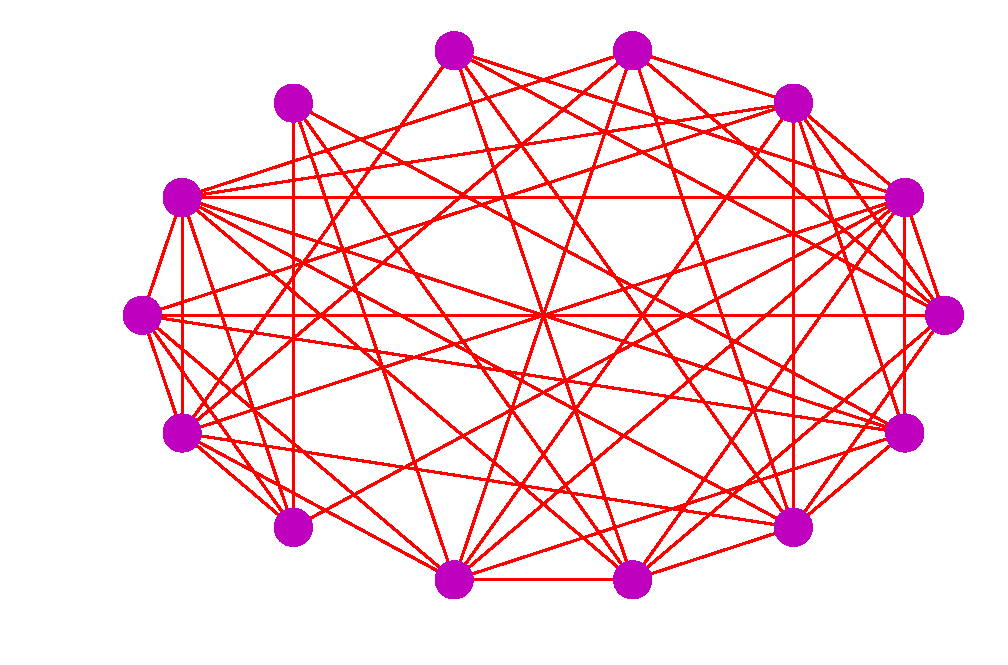
\includegraphics[scale=0.45]{foo}
\caption{}
\end{figure}

\begin{figure}[h!]
\centering
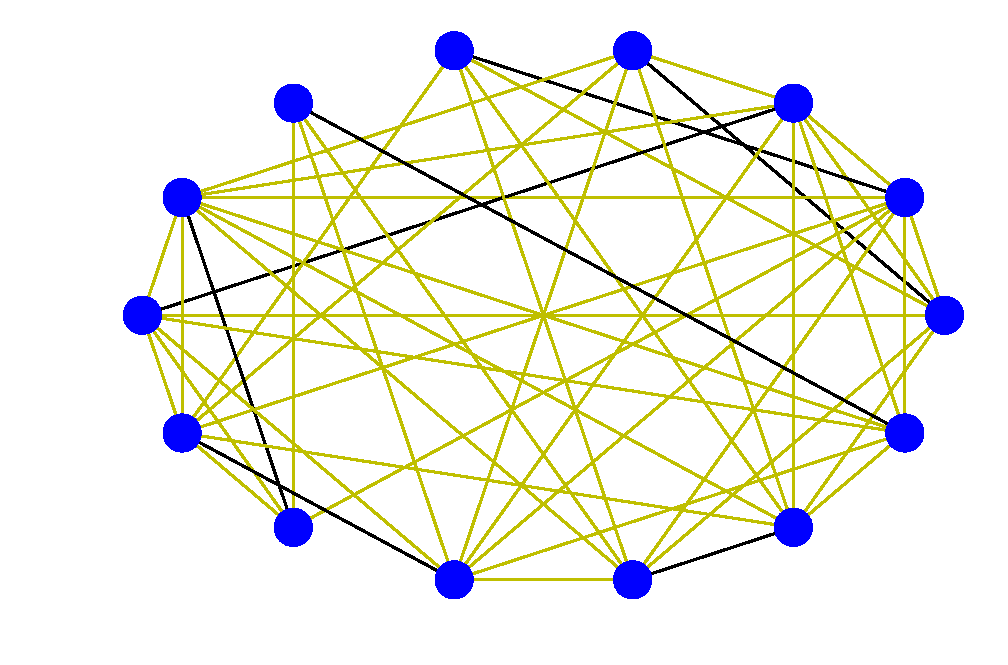
\includegraphics[scale=0.45]{foo1}
\caption{}
\end{figure}

\newpage
\begin{pythone}
# Si simplemente utilizamos draw, el dibujo es algo mas caotico.
networx.draw(G)
\end{pythone}

\begin{figure}[h!]
\centering
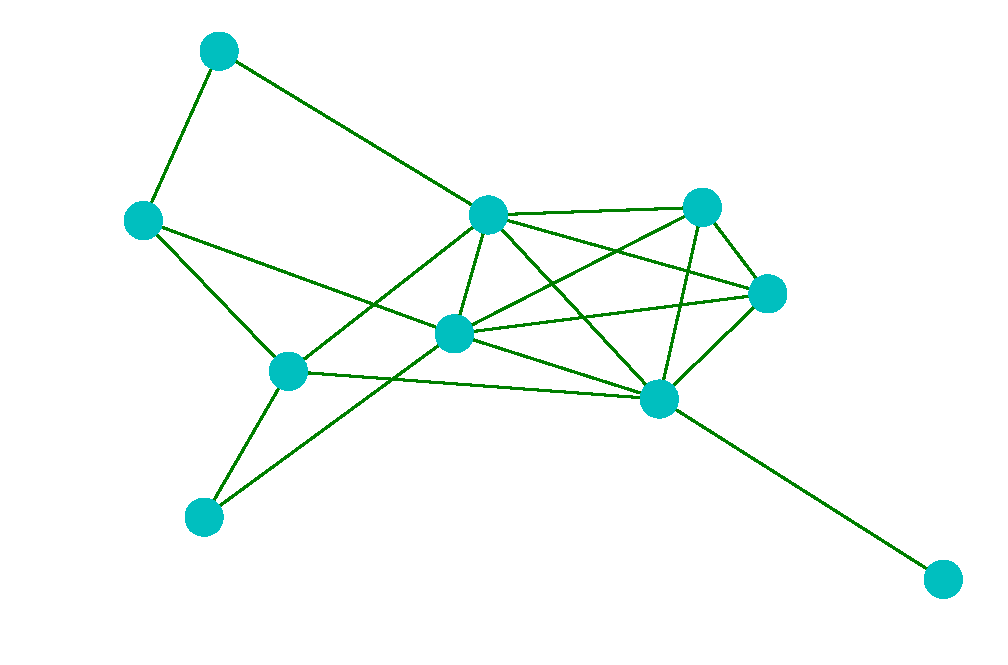
\includegraphics[scale=0.55]{foo2}
\caption{}
\end{figure}


\begin{pythone}
# Tambien tenemos una opcion para utilziar el algoritmo de Kamada-Kawai para dibujar redes.
networx.draw_kamada_kawai(G)
\end{pythone}

\begin{figure}[h!]
\centering
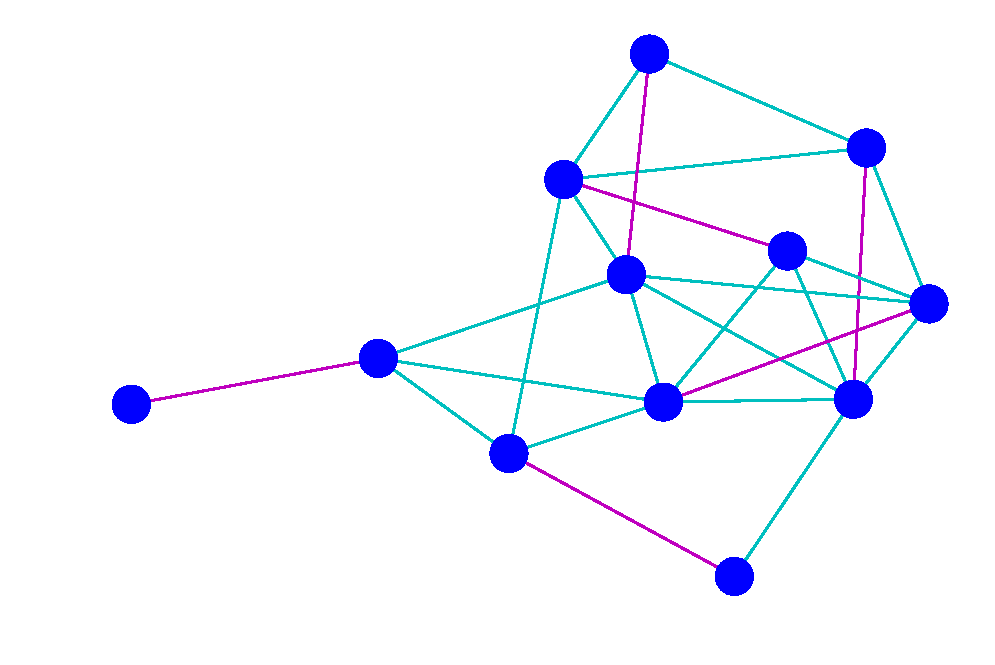
\includegraphics[scale=0.55]{foo3}
\caption{}
\end{figure}

\newpage
\subsection{SCIP y soluciones no soportadas}
En un problema de Programación Lineal las soluciones proporcionadas por el método del simplex, en caso de existir, han de situarse en los vértices de la envolvente convexa de nuestro conjunto factible. Cuando trabajamos con problemas multiobjetivo no tiene por qué existir una solución que minimice simultáneamente todas las funciones objetivo. En este sentido, tenemos las denominadas soluciones de Pareto, es decir, aquellas que no pueden ser mejorada en alguna de sus funciones componentes sin empeorar otra. El conjunto de soluciones de Pareto, o vectores Pareto eficientes, se conoce como frontera de Pareto. Este tipo de soluciones se pueden conseguir, en el caso biobjetivo, tal y como hemos planteado en la sección 3.1.6. Sin embargo, aunque las funciones objetivo y resticciones sean lineales pueden existir soluciones de Pareto que no estén en la frontera de la envolvente convexa de nuestro conjunto factible. Estas soluciones se conocen como no soportadas.

Con el software Gurobi no podemos encontrar las soluciones no soportadas, por lo que tendermos que utilizar el software SCIP, y en particular una de sus aplicaciones, PolySCIP. Este solver solo acepta un tipo determinado de extensión denominada .mop. Nosotros adjuntamos el siguiente código en el que, dado un grafo $G$ y funciones de costo $c_1$ y $c_2$, se genera el archivo .mop del problema de matching asociado escrito con la formulación de Programación Entera.

\begin{pythone}
# En este codigo vamos a implementar un sencillo programa para convertir un grafo G y dos vectores c1, c2 en un fichero .mop para que PolySCIP pueda resolverlo
import networkx as nx
import random
import math

def pytoscip(name,sense, G, costes):
    
    obj = list(enumerate(costes))
    aristas = list(enumerate(G.edges()))
    # Creamos el archivo
    file = open(name + ".mop","w") 
    file.write("NAME          EX1\n") 
    
    # El pararametro sense puede ser MAX o MIN
    file.write("OBJSENSE\n")    
    file.write(" " + sense + "\n") 

    # Añadimos el las funciones objetivo y restricciones
    file.write("ROWS\n")
    
    # Funciones objetivo
    for (i,s) in obj:
        file.write(" N  Obj" + str(i) + "\n")  
           
    # Restricciones de grado
    for v in G:
        file.write(" E  Eqn" + str(v) + "\n")
        
    # A continuacion pasamos a las columnas
    file.write("COLUMNS\n")
    
    for (i,(a,b)) in aristas:
        m1,m2,m3 = len(str(i)), len(str(a)), len(str(b))
        l1 = 8-m1
        l2 = 18-m2
        l3 = 18-m3
        inicio = 4*" " + "x#" + str(i) + l1*" " 
        file.write(inicio + "Eqn" + str(b) + l3*" " + "1\n")
        file.write(inicio + "Eqn" + str(a) + l2*" " + "1\n")
        for (k,s) in reversed(obj):
            m4 = str(s[i])
            l4 = 19 - len(str(k)) -len(m4)
            file.write(inicio + "Obj" + str(k) + l4*" " + m4 + "\n")
           
    # Los coeficientes
    file.write("RHS\n")
    for v in G:
        l = len(str(v))
        m = 18-l
        file.write(4*" " + "RHS" + 7*" " + "Eqn" + str(v) + m*" " + "1\n")    
    # Cotas inferiores 
    file.write("BOUNDS\n")        
    for (i,q) in aristas:
        l = len(str(i))
        m = 19-l
        file.write(" LI BOUND" + 5*" " + "x#" + str(i) + m*" " + "0\n")    
    file.write("ENDATA")
    file.close()
\end{pythone}

\newpage
\section{Resultados computacionales}
A continuación presentamos los resultados computacionales obtenidos. Utilizando los códigos anteriores, vamos a generar una serie de grafos aleatorios con un cierto número de vértices y funciones de coste aleatorias. Resolveremos entonces los problemas de emparejamiento asociados y reportaremos ciertos resultados relacionados. En la siguiente tabla tenemos las siguientes variables.
\begin{itemize}
\item $N$ es el numero de vértices considerados.
\item $I$ es el número de grafos aleatorios que generamos, es decir, los casos que estudiamos para cada $N$.
\item $Var$ es el número medio de aristas que tienen los grafos considerados y, por tanto, el número medio de variables que tienen los problemas.
\item $S.GH$, $S.PE$ y $S.Match$ es el número medio de iteraciones del simplex que se utilizan respectivamente durante el método de Grötschel-Holland, usando Programación Entera y usando el simplex sobre la formulación del poliedro del matching.
\item Análogamente $T.GH$, $T.PE$ y $T.Match$ son los tiempos medios en los que cada método ha resuelto los correspondientes problemas.
\item $Exp.B.B$ es el número de nodos de branch and cut explorados cuando utilizamos Programación Entera.
\end{itemize} 
Una vez que el tiempo medio necesario para resolver un problema es superior a 30 segundos, dejamos de utilizar dicho método y todos los valores pasan a ser $0$. Observamos que para grafos con 18 vértices ya comienza a ser costroso utilizar la formulación de Edmonds debido a que introducimos un número exponencial de restricciones.
\begin{table}[ht]
\centering
\begin{tabular}{rrrrrrrrrr}
  \hline
N & I & Var & S.GH & S.PE & S.Match & T.PE & T.GH & T.Match & Exp.B.B \\ 
  \hline
10 & 10 & 21.40 & 4.90 & 5.60 & 8.50 &   0.01 & 0.02 & 0.04 & 0.10 \\ 
16 & 10 & 59.40 & 8.90 & 13.90 & 17.80 & 0.01 & 0.03 & 3.34 & 0.00 \\ 
18 &  5 & 75.60 & 13.40 & 17.60 & 20.20& 0.02 & 0.03 & 17.46 & 0.20 \\ 
 \hline
40 & 10 & 389.00 & 36.50& 43.50 & 0.00 & 0.04 & 0.05 & 0.00 & 0.50 \\ 
60 & 10 & 886.20 & 56.40& 62.00 & 0.00 & 0.10 & 0.11 & 0.00 & 0.40 \\ 
100 & 10 & 2469.80 & 102.80 & 108.80 & 0.00 & 0.24 & 0.22 & 0.00 & 0.40 \\ 
120 &   10 & 3551.80 & 109.20 & 113.60 & 0.00 & 0.33 & 0.32 & 0.00 & 0.00 \\ 
150 &   10 & 5551.20 & 153.40 & 160.60 & 0.00 & 0.56 & 0.45 & 0.00 & 0.00 \\ 
170 &   10 & 7164.60 & 167.80 & 174.40 & 0.00 & 0.83 & 0.60 & 0.00 & 0.20 \\ 
200 &   10 & 10034.00 & 201.80 & 204.00 & 0.00 & 1.31 & 0.80 & 0.00 & 0.20 \\ 
  \hline
 \end{tabular}
 \end{table}
\begin{table}[h]
\centering
\begin{tabular}{rrrrrrrrrr}
  \hline
N & I & Var & S.GH & S.PE & S.Match & T.PE & T.GH & T.Match & Exp.B.B \\ 
  \hline 
  220 &   5 & 12033.00 & 210.40 & 219.40 & 0.00 & 1.50 & 0.93 & 0.00 & 0.00 \\ 
  250 &   5 & 15529.20 & 253.80 & 258.00 & 0.00 & 2.65 & 1.28 & 0.00 & 0.40 \\ 
  270 &   5 & 18139.40 & 286.80 & 291.40 & 0.00 & 4.09 & 1.55 & 0.00 & 0.60 \\ 
290 &     5 & 20955.60 & 290.00 & 300.20 & 0.00 & 4.67 & 1.73 & 0.00 & 0.60 \\ 
  300 &   5 & 22416.80 & 298.00 & 306.80 & 0.00 & 4.75 & 1.78 & 0.00 & 0.40 \\ 
320 &   5   & 25466.80 & 345.40 & 398.00 & 0.00 & 10.20 & 2.12 & 0.00 & 0.60\\
  350 &   5 & 30601.80 & 385.80 & 390.80 & 0.00 & 10.84 & 2.51 & 0.00 & 0.60\\
  370 &   5 & 34050.60 & 387.20 & 399.00 & 0.00 & 11.00 & 2.73 & 0.00 & 0.40\\
  400 &   5 & 39902.80 & 426.60 & 432.00 & 0.00 & 17.09 & 3.44 & 0.00 & 0.60 \\ 
   \hline
 
\end{tabular}
\end{table}
\newpage
A continuación, presentamos algunas gráficas de los resultados anteriores.
\begin{figure}[h]
\centering
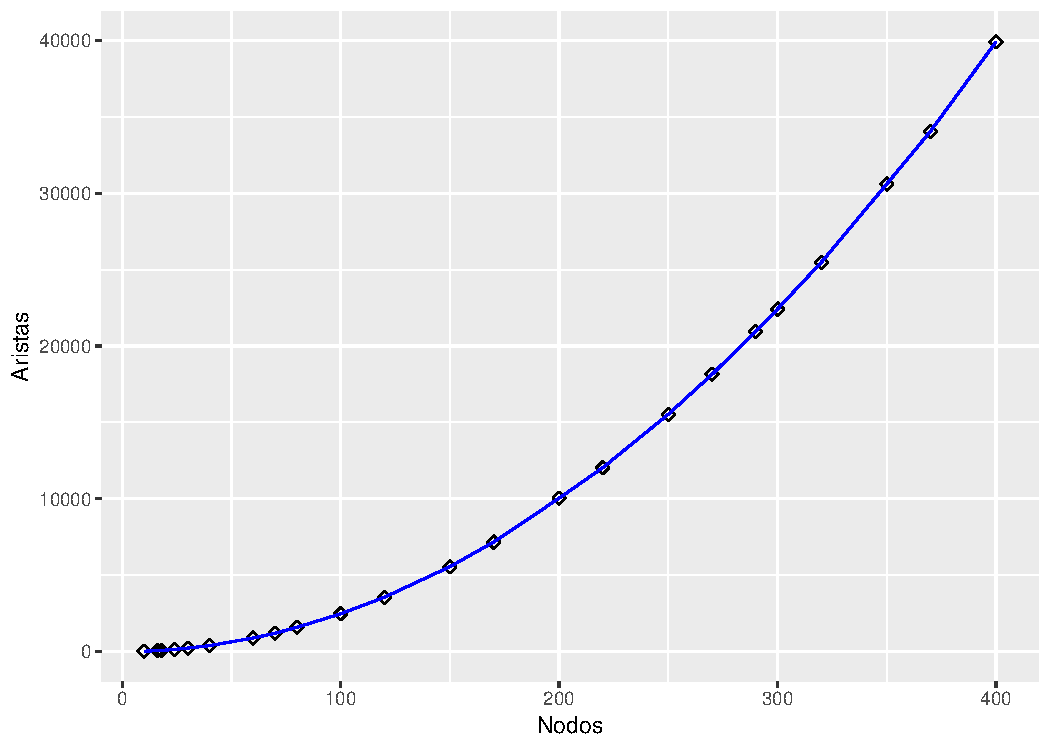
\includegraphics[scale=0.75]{plot1}
\caption{Aristas frente Nodos}
\end{figure}

En la primera gráfica tratamos de representar la cantidad de aristas frente a los nodos. Dado que como parámetro del grafo de Erdös-Rényi hemos tomado $p=0.5$ y el número posible de aristas es $N(N-1)/2$, hemos dibujado por debajo los puntos de $N(N-1)/4$, es decir, el número de puntos esperados. Como vemos, la gráfica se superpone.

A continuación comparamos el número de iteraciones del método del simplex y el tiempo de computación frente al número de nodos en para el algortimo de Grötschel-Holland y para los métodos de Gurobi para resolver Programación Entera.

\begin{figure}[h!]
\centering
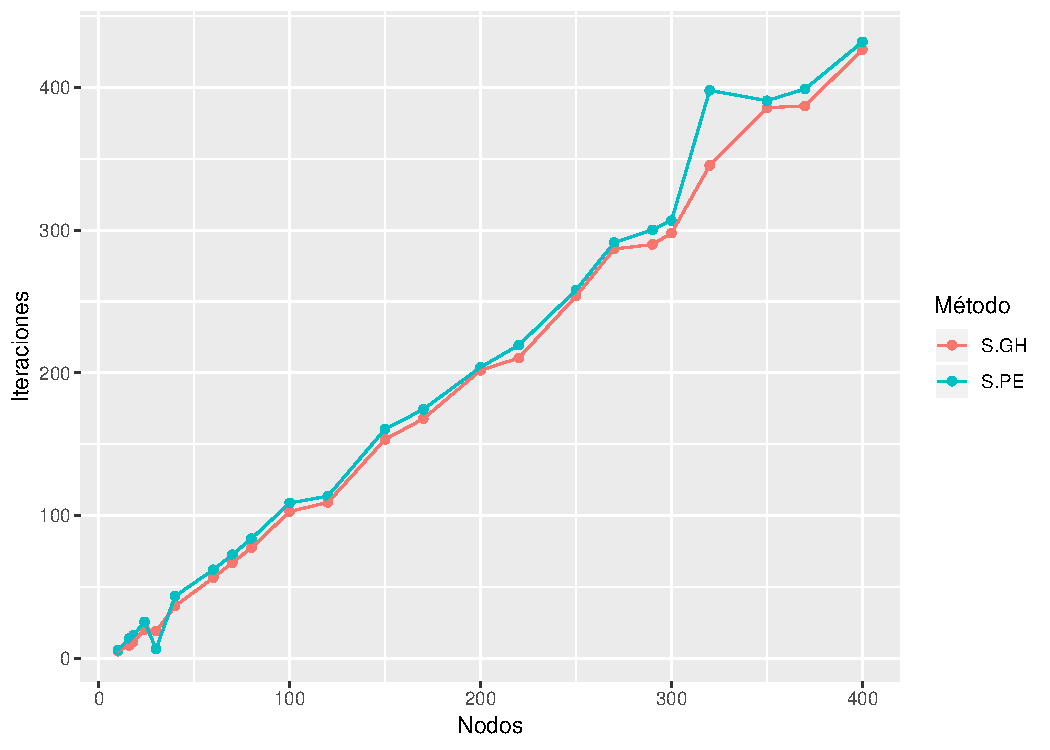
\includegraphics[scale=0.75]{plot2}
\caption{Iteraciones del Simplex frente a Nodos}
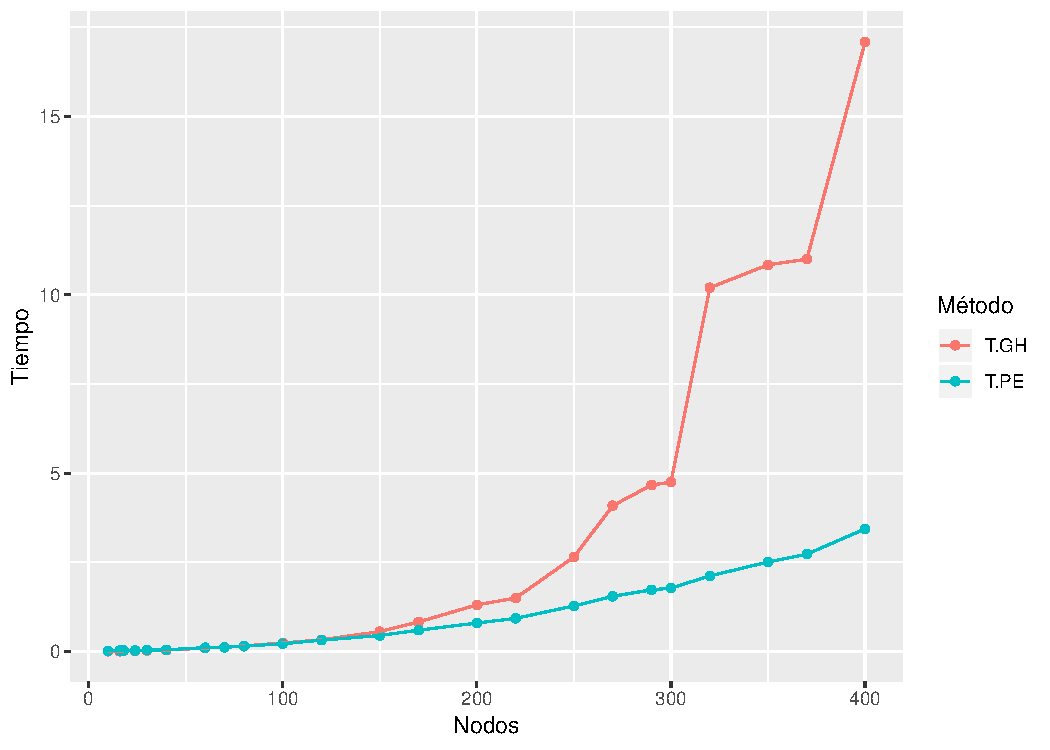
\includegraphics[scale=0.75]{plot3}
\caption{Tiempo de computación en segundos frente a Nodos}
\end{figure}

\section{Reoptimización}
Al desactivar el pre-solve, nos aseguramos que tras cambiar la función objetivo se parte de la misma base óptima. Ya explicamos anteriormente cómo conseguimos la variación del parámetro y la solución. Veamos un ejemplo.
\begin{figure}[h!]
\centering
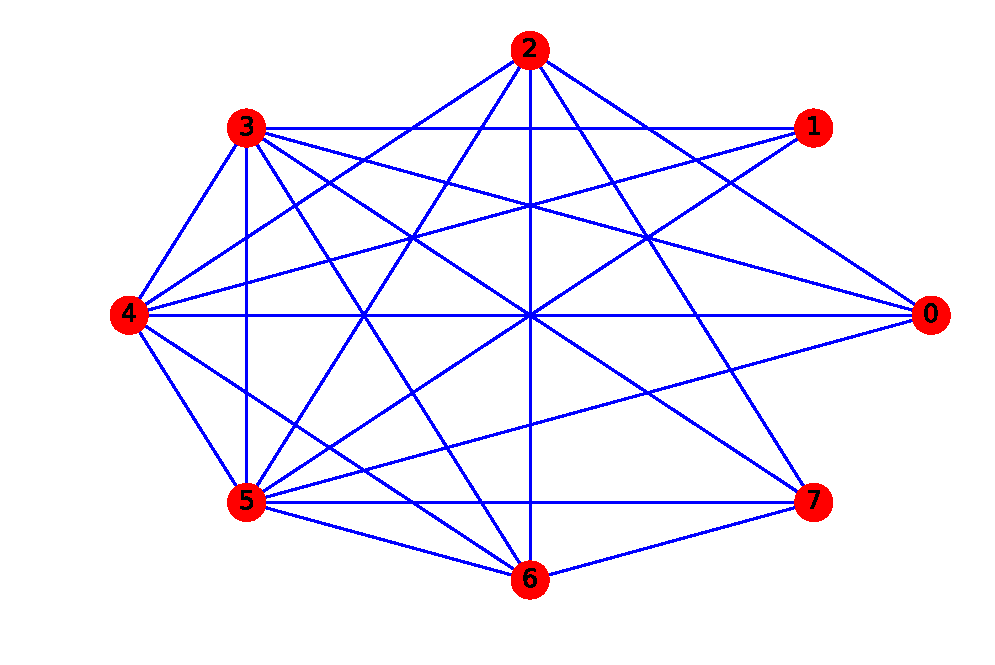
\includegraphics[scale=0.5]{opt}
\caption{Grafo inicial}
\end{figure}

Partimos de las funciones de coste de las aristas (las cuáles están ordenadas según el orden lexicográfico):
\begin{pythone}
c1 = [0.77783098, 0.26790423, 0.22276086, 0.82550433, 0.552517, 0.18884415, 0.01789486, 0.00243447, 0.04742837, 0.94171732, 0.76081629, 0.70075895, 0.16148063, 0.62424824, 0.95096634, 0.16806133, 0.88617127, 0.57725367, 0.17168492, 0.85295435]
c2 = [0.64317771, 0.56083433, 0.55490255, 0.29773688, 0.08169206, 0.89175246, 0.56850518, 0.57067846, 0.13329401, 0.15793078, 0.41082069, 0.13778612, 0.39161058, 0.34617111, 0.25853244, 0.79687483, 0.58816817, 0.00892943, 0.18819747, 0.52953081]
\end{pythone}
Utilizando el método presentado en la subseción 3.1.6. para la reoptimización, comenzamos resolviendo para $\lambda=0$ calculamos el máximo valor de $\lambda$ para el cuál la base actual sigue siendo óptima. Tras modificar la función objetivo y reoptimizar, obtenemos una solución que puede volver a ser la misma o no. Si no lo fuese, capturamos el valor de $\lambda$ y la solución. Obtenemos así que para $\lambda\in [0,1]$ encontramos 3 soluciones distintas para valores límite de $\lambda \in \{0,0.5814,0.6626\}$.

En un análisis posterior, resolvemos el mismo problema usando Programación Entera para una regilla de valores $\lambda$ entre $0$ y $1$ con paso $0.1$. Así obtenemos lo que cabría esperar, para $\lambda \leq 0.5$ obtenemos la primera solución, para $\lambda = 0.6$ obtenemos la segunda solución y para $0.7 \leq \lambda \leq 1$ obtenemos la tercera solución. Presentamos una representación gráfica de los distintos emparejamientos asociados a cada $\lambda$. 
\begin{figure}[h!]
\centering
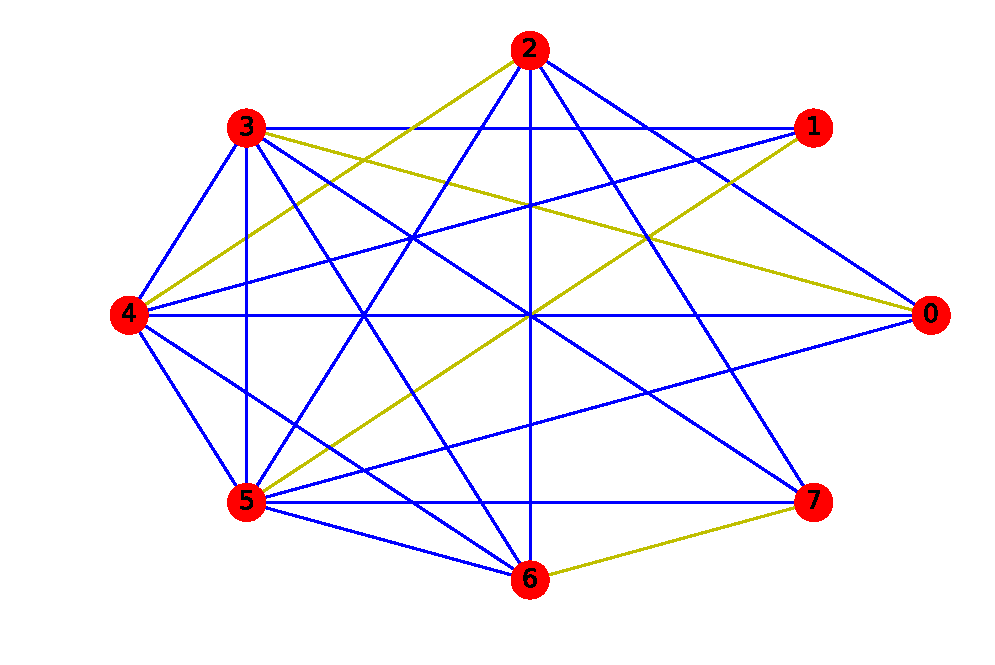
\includegraphics[scale=0.5]{opt2}
\caption{Solución para $\lambda=0$}
\end{figure}


\begin{figure}[h!]
\centering
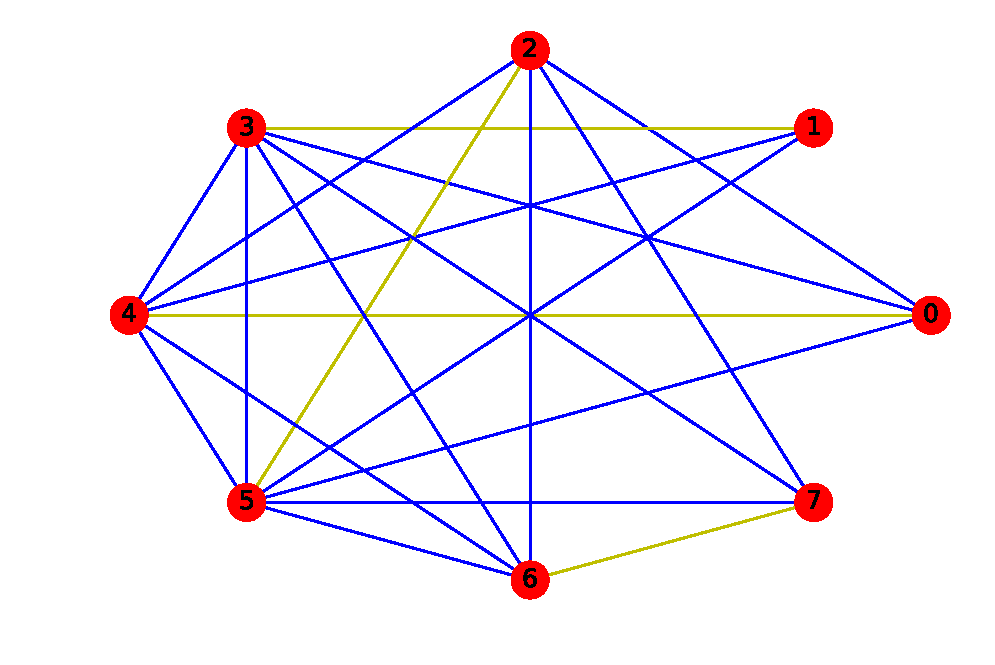
\includegraphics[scale=0.5]{opt3}
\caption{Solución para $\lambda=0.5814219436621$}
\end{figure}


\begin{figure}[h!]
\centering
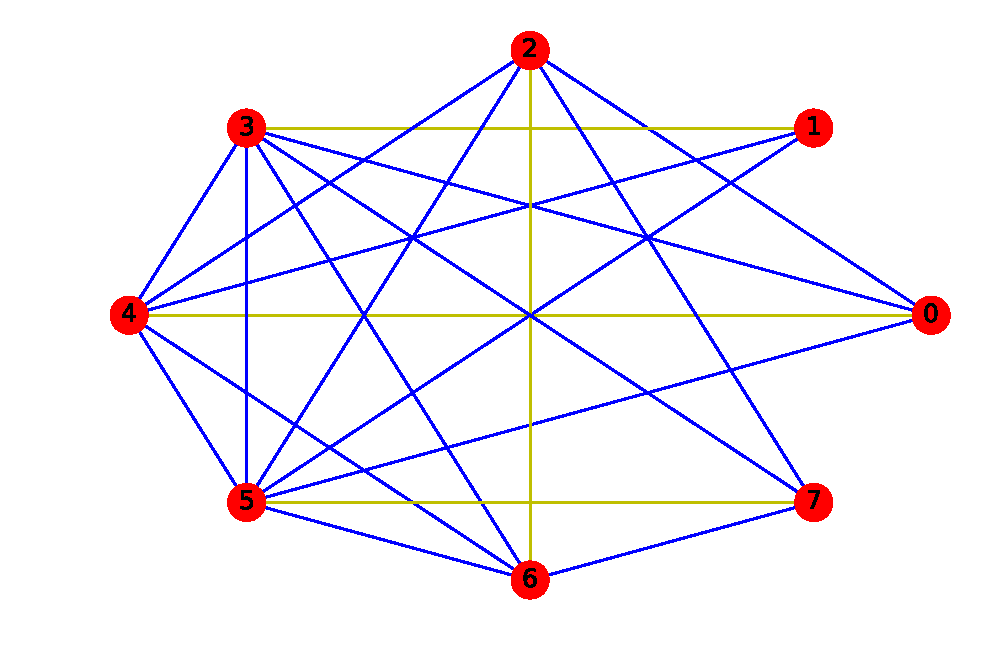
\includegraphics[scale=0.5]{opt4}
\caption{Solución para $\lambda=0.6626459613176332$}
\end{figure}
\newpage
Reportamos también el siguiente análisis. Para un cierto número $N$ de vértices, generamos 5 grafos y sendas funciones de costo. A continuación usando las mismas técnicas que usamos anteriormente, calculamos el número de soluciones soportadas, es decir, aquellas que están en la frontera del poliedro y que conseguimos obteniendo al variar $\lambda \in [0,1]$. Mostramos el número promedio de soluciones para cada $N$ considerado.
\begin{table}[ht]
\centering
\begin{tabular}{rr}
  \hline
  N & Sols \\ 
  \hline
20 & 10.00 \\ 
40 & 19.80 \\ 
60 & 31.00 \\ 
80 & 45.60 \\ 
100 & 51.60 \\ 
120 & 63.80 \\ 
140 & 68.00 \\ 
   \hline
\end{tabular}
\end{table}

Por desgracia es realmente costoso tratar de buscar las soluciones interiores para el problema biobjetivo, de manera que para grafos de 30 nodos ya resulta relativamente costoso en un ordenador usual. En nuestro caso, para ciertos valores de $N$ entre $16$ y $30$, vamos a generar 5 problemas para estudiar el comportamiento medio de las soluciones soportadas frente a no soportadas. La función para generar grafos aleatorios toma en este caso el parámetro $p=0.7$. 

En la siguiente tabla encontramos el número $N$ de vértices de los grafos considerados, la Media Total de soluciones (soportadas y no soportadas), la media de soluciones no soportadas y la media de las soluciones soportadas frente al total.
\begin{table}[ht]
\centering
\begin{tabular}{rrrr}
  \hline
N & Media Total & Media No Sop & Media Porcentaje \\ 
  \hline
  14 & 9.40 & 4.60 & 45.39 \\ 
  16 & 15.80 & 10.20 & 63.72 \\ 
  18 & 18.80 & 10.40 & 55.90 \\ 
  20 & 22.60 & 14.80 & 65.31 \\ 
  22 & 30.00 & 19.20 & 63.55 \\ 
  24 & 39.20 & 27.00 & 68.81 \\ 
  26 & 40.00 & 29.40 & 72.81 \\ 
  28 & 53.80 & 38.60 & 73.05 \\ 
  30 & 63.00 & 48.40 & 76.91 \\ 
   \hline
\end{tabular}
\end{table}

Adjuntamos además algunas gráficas de la tabla anterior.

\begin{figure}[h!]
\centering
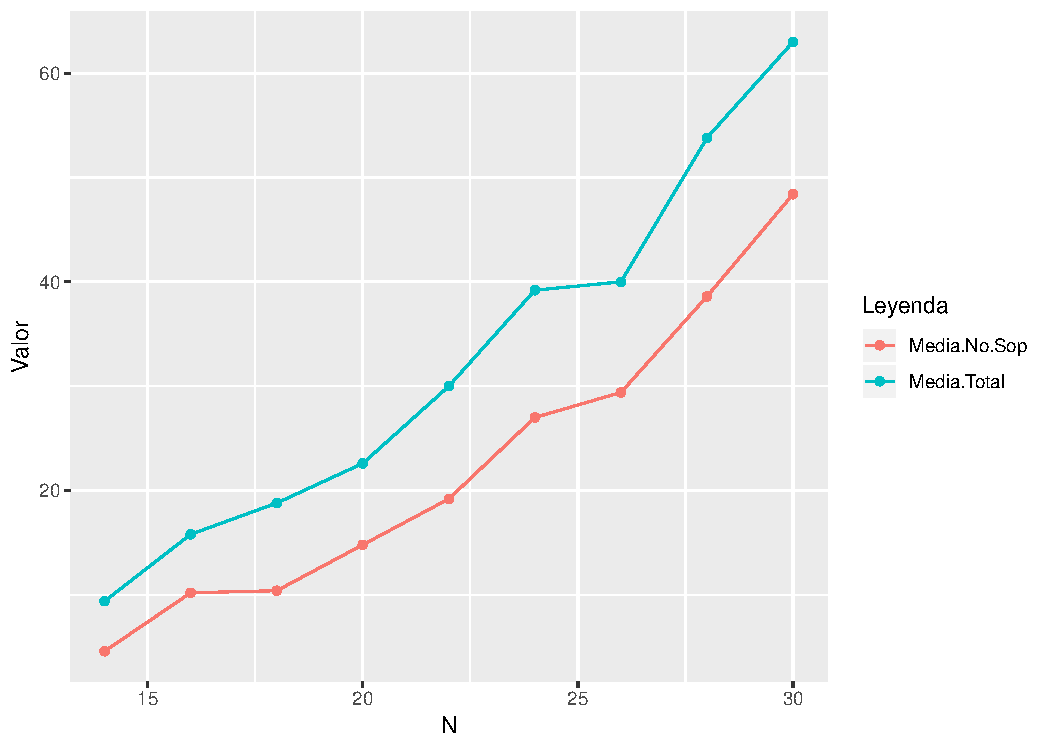
\includegraphics[scale=0.7]{plot10}
\caption{Número medio de solucones frente a nodos}
\end{figure}


\begin{figure}[h!]
\centering
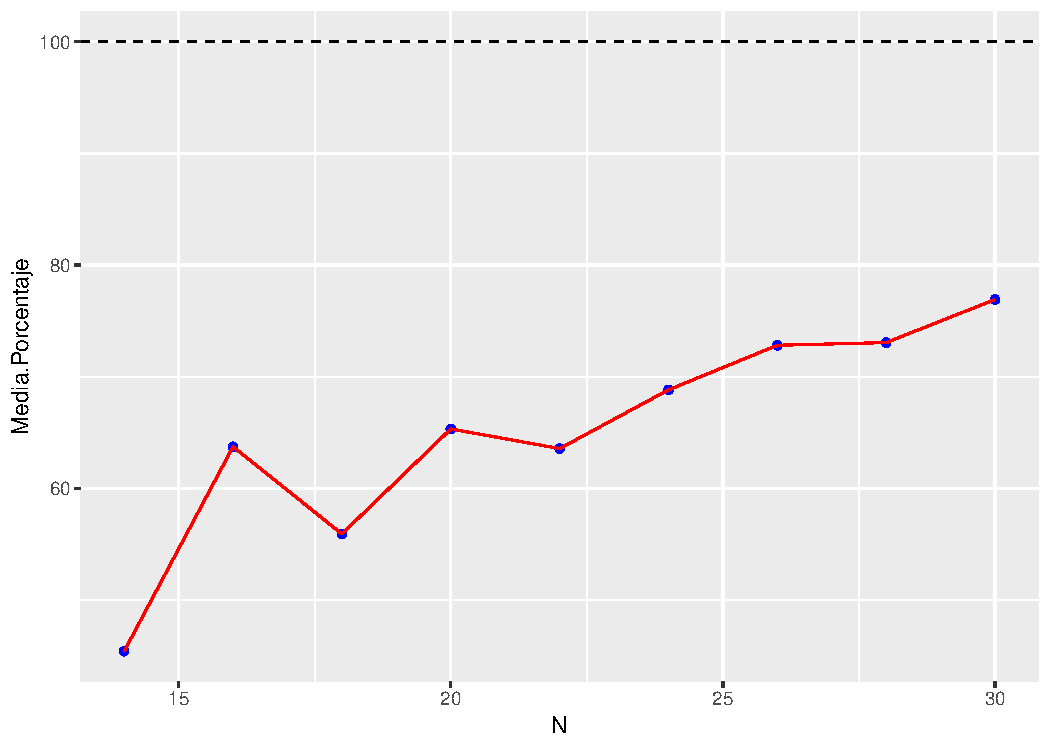
\includegraphics[scale=0.7]{plot11}
\caption{Media de porcentajes frente a nodos}
\end{figure}
\begin{thebibliography}{9}
\bibitem{edmond} 
Edmonds, J. (1965). Maximum matching and a polyhedron with 0, 1-vertices. Journal of Research of the National Bureau of Standards B, 69, 125--130. 

\bibitem{kuhn}
Kuhn, H. W. (1955), The Hungarian method for the assignment problem. Naval Research Logistics, 2: 83-97. doi:10.1002/nav.3800020109
  
\bibitem{holland} 
Grötschel, M.; Holland, O. Mathematical Programming (1985) 33: 243. https://doi.org/10.1007/BF01584376

\bibitem{pruebaed} 
Schrijver, Alexander. (1983). Short proofs on the matching polyhedron. Journal of Combinatorial Theory, Series B. 34. 104-108. 10.1016/0095-8956(83)90011-4. 
 
\bibitem{balltab}
Ball, M. O.,  Taverna, R. (1985). Sensitivity analysis for the matching problem and its use in solving matching problems with a single side constraint. Annals of Operations Research, 4(1), 25-56.

\bibitem{papa}
Papadimitriou, C.H.; Steiglitz, K. (1998), Combinatorial optimization: algorithms and complexity, Mineola, NY: Dover, pp.308-309.

\bibitem{nico}
Nicos Christofides, Worst-case analysis of a new heuristic for the travelling salesman problem, Report 388, Graduate School of Industrial Administration, CMU, 1976

\bibitem{inte}
George L. Nemhauser and Laurence A. Wolsey. 1988. Integer and Combinatorial Optimization. Wiley-Interscience, New York, NY, USA.
\bibitem{edmon2}
J. Edmonds, “Paths, Trees, and Flowers,” Can. J. Math., 17,449-467 (1965).

\bibitem{edmon3}
Pulleyblank, William and Edmonds, Jack. (1970). Facets of 1-Matching Polyhedra. 10.1007/BFb0066196. 

\bibitem{derigs}
Derigs, U. (1981), A shortest augmenting path method for solving minimal perfect matching problems. Networks, 11: 379-390. doi:10.1002/net.3230110407

\bibitem{webber}
Weber, G. M. (1981), Sensitivity analysis of optimal matchings. Networks, 11: 41-56. doi:10.1002/net.3230110105

\bibitem{rao}
Padberg, Manfred W., and M. R. Rao. “Odd Minimum Cut-Sets and b-Matchings.” Mathematics of Operations Research, vol. 7, no. 1, 1982, pp. 67–80. JSTOR, www.jstor.org/stable/3689360.

\bibitem{adam}
Letchford, Adam;  Reinelt, Gerhard; Theis, Dirk Oliver. (2004). A Faster Exact Separation Algorithm for Blossom Inequalities. 10.1007/978-3-540-25960-215. 

\bibitem{sepa}
M. Grötschel, L. Lovász, and A. Schrijver. The ellipsoid method and its
consequences in combinatorial optimization. Combinatorica, 1(2):169-197, 1981

\bibitem{scip}
R. Borndörfer, S. Schenker, M. Skutella, T. Strunk: PolySCIP.
Mathematical Software - Proceedings of ICMS 2016, G.-M. Greuel, T. Koch, P. Paule, A. Sommese (Eds.),
Lecture Notes in Computer Science Vol. 9725, ISBN: 978-3-319-42431-6

\bibitem{gurobi}
Gurobi Optimization, Inc. Gurobi Optimizer Reference Manual Version 3.0. Houston, Texas: Gurobi Optimization, April 2010.
\end{thebibliography}
\end{document} 
